% ============================================================
% experiments/exp01_smoke/report.tex
% exp01_smoke 实验报告 —— 自包含「实验设置 + 主要结果 + 图表」
%
% 数据来源（路径均相对本文件）：
%   results/metrics.json   逐周期与汇总指标
%   results/solution.json  场景、机群、任务、交付航次
%   results/figures/       图产物（17 个）
%   results/tables/        结果表（exp01_tables.tex / .pdf）
%
% 编译：latexmk -xelatex report.tex     （ctex 需 xelatex）
% ============================================================
\documentclass[a4paper,11pt]{article}

\usepackage[margin=2.3cm]{geometry}
\usepackage{graphicx}
\usepackage{booktabs}
\usepackage{caption}
\usepackage{float}
\usepackage{amsmath,amssymb}
\usepackage{array}
\usepackage[table]{xcolor}
\usepackage[hidelinks]{hyperref}
\usepackage{ctex}
\usepackage{seqsplit}

\graphicspath{{results/figures/}}

% 长文件名/命令行：允许在任意字符间断行，避免 Overfull
\newcommand{\fname}[1]{{\ttfamily\seqsplit{#1}}}

\captionsetup{font=small,labelfont=bf,skip=6pt}
\setlength{\parskip}{4pt}
\renewcommand{\arraystretch}{1.15}
\setlength{\tabcolsep}{5pt}

\title{\textbf{exp01\_smoke 实验报告}\\[6pt]
\large 动态任务分配两阶段框架的真实地形滚动时域验证}
\author{}
\date{实验日期：2026--10--16\quad 随机种子：seed = 42\quad 实际运行周期：8}

\begin{document}
\maketitle

\begin{abstract}
\noindent 本报告记录 exp01\_smoke 实验的设置与结果。实验在真实 DEM 地形（SRTM/ASTER 级高程数据，
200\,m 采样）上构建含 10 架无人机、8 个机巢、60 个带时间窗动态任务的场景，采用
\textbf{任务选择 + MUAS 求解} 的两阶段分配框架与滚动时域调度，任务分三个周期（30/10/20）到达，
以收敛早停终止。结果显示：60 个任务全部完成（完成率 100\%），
\textbf{违约交付（废飞）0 次、超期淘汰 0 个、静态不可达 0 个}；
按时率 80\%（迟到 12 个，平均迟到 691\,s），
平均等待 720\,s，吞吐 7.5 任务/周期，总航程 1781.0\,km，累计奖励 291.90。
本报告同时明确各项指标的计算口径，特别是逐周期正确执行率受空转周期影响的定义差异。
\end{abstract}

\tableofcontents
\newpage

% ============================================================
\section{实验设置}
% ============================================================

\subsection{实验目标与评价口径}

实验目标\textbf{不是}追求完成率，而是验证框架在\textbf{持续任务到达下尽可能多且正确地完成任务}
的长程执行能力。依据该目标，本实验采用以下核心指标口径：

\begin{itemize}
  \item \textbf{累计正确完成数}：真正交付执行的任务数（含迟到交付）；
  \item \textbf{违约交付（废飞）}：被判物理不可行、无人机已飞出航程且位置已更新、
        但任务解绑回池不计完成的事件。总航程下降若以此换来则为净亏损，须与吞吐同权报告；
  \item \textbf{超期淘汰}：deadline 已过仍在池中、被过期出池的任务数，
        对物理可行任务是兜底失灵的信号，应趋近于 0；
  \item \textbf{静态不可达}：所有机巢往返航程均超过满电可及范围的任务
        （过于偏远，属物理约束，是唯一合法的未完成原因），入池时一次性判定出池；
  \item \textbf{吞吐}：累计完成任务数 / 实际运行周期数；
  \item \textbf{每周期正确执行率}与\textbf{按时率}：衡量执行质量（口径见 \S 2.3）。
\end{itemize}

\subsection{场景与地形}

实验区域位于青藏高原（约 N29$^\circ$/E091$^\circ$，拉萨一带），地形高程数据取自
\fname{ASTGTMV003\_N29E091\_dem.tif}，采样步长 200\,m，有效格网 508 $\times$ 575。
本地平面坐标系原点取 $(\text{lat}_0,\text{lon}_0)=(29.5222025,\,91.47933125)$，
8 个机巢的地理坐标据此投影得到，场景范围约 $101.6 \times 115.0$\,km。

\textbf{距离口径}：所有距离一律采用\textbf{垂直切面 DEM 三维航程}（考虑地形起伏的
空间直线距离），而非二维平面欧氏距离；凡由距离推导时间（ETA、时间窗判定、航程约束、
边际插入估计）均由统一的代价提供者计算，保证全链路口径一致。
机巢间跨度约 90\,km。

\subsection{机群、机巢与任务}

\begin{table}[H]
\centering
\caption{实验主体参数}
\label{tab:entities}
\footnotesize
\begin{tabular}{@{}ll>{\raggedright\arraybackslash}p{7.6cm}@{}}
\toprule
参数 & 取值 & 说明 \\
\midrule
无人机数量 & 10 架 & 初始驻留：UAV $i \to$ 机巢 $i \bmod 8$ \\
机巢数量 / 容量 & 8 个 / 每巢 4 架 & 共 32 个泊位，机巢容量为硬约束 \\
满电航程 & 80\,km & 每周期末在机巢充电恢复至满电 \\
巡航速度 & 15\,m/s & 所有航段统一 \\
任务总数 & 60 个 & 周期 1/2/3 分别到达 30/10/20 \\
任务时间窗 & 周期相关 & $\text{latest}=\text{到达时刻}+U(4.5,9.0)\times\text{周期长}$ \\
\bottomrule
\end{tabular}
\end{table}

任务属性包括三维坐标、奖励值、最早/最晚可服务时刻与状态。
任务奖励的量级约为 7.0（本批任务最小奖励 7.0156），
时间窗跨度按 DEM 航时标定为 4.5--9.0 个周期。

\subsection{滚动时域与两阶段求解流程}

仿真按滚动时域推进，每周期执行一次完整的分配—执行循环：

\begin{enumerate}
  \item \textbf{任务选择（selection）}：按「优先级 $\to$ 可行性 $\to$ 边际收益」三级顺序，
        从当前任务池中选出本周期参与分配的任务集，并挑出可出动的无人机；
  \item \textbf{MUAS 求解（muas）}：以 DMDE（离散多目标差分进化）搜索
        \textbf{无人机归属 + 访问顺序}；\textbf{终点机巢不进编码}，
        而由内层最小费用流在容量约束下精确求解后解码，返航代价计入目标；
  \item \textbf{修复链}：对求解结果依次执行合并、剔除、航程修复与终点机巢选择，
        迭代至定点收敛，再执行覆盖补全与时间窗重排；
  \item \textbf{执行与状态更新}：无人机按航次起飞，消耗航程、更新位置，周期末在机巢充电。
\end{enumerate}

DMDE 参数：种群规模 50，迭代代数 100（论文主口径，500 代另作敏感性对照）；
标量化采用字典序 big-M 形式（收益优先，航程与惩罚为次目标），
次目标权重 $\lambda = 1.0\times10^{-4}$ 收益当量/米。
早停条件：任务池规模连续 4 个周期不变即判定收敛。

\subsection{约束口径与完成判定协议}

\begin{itemize}
  \item \textbf{航程约束}：$\text{往返航程} \le \text{margin}\times\text{剩余航程}$，
        $\text{margin}=1.0$（满电物理上限），与完成闸门同口径；
  \item \textbf{时间窗}：预筛阶段\textbf{不}以时间窗作为参选资格，
        迟到由适应度定价而非直接拒绝；
  \item \textbf{完成判定}：仅当任务被判\textbf{物理不可行}
        （航程/续航/终点机巢/结构类违约）时才弹回任务池、不计完成；
        \textbf{迟到不算废飞}——迟到交付计入完成，奖励按
        \[
          \text{eff} = R \times \max\!\left(0,\; 1 - \frac{L}{W}\right)
        \]
        折减，其中 $L$ 为迟到时长，$W=\text{late\_reward\_decay\_seconds}=600$\,s。
\end{itemize}

% ============================================================
\section{主要结果}
% ============================================================

\subsection{汇总指标}

\begin{table}[H]
\centering
\caption{exp01\_smoke 汇总指标（seed = 42，实际 8 周期）}
\label{tab:summary}
\small
\begin{tabular}{lrll}
\toprule
指标 & 数值 & 口径 / 备注 \\
\midrule
到达任务数            & 60        & 周期 1/2/3 分别 30/10/20 \\
\textbf{完成任务数}   & \textbf{60} & 完成率 100\%（含迟到交付） \\
\textbf{违约交付（废飞）} & \textbf{0} & 物理不可行弹回，目标为 0 \\
\textbf{超期淘汰}     & \textbf{0} & deadline 已过仍在池中 \\
静态不可达            & 0         & 所有机巢往返 $>$ 满电航程 \\
按时率                & 80.0\%    & 48/60；按任务加权 \\
迟到任务数            & 12        & 完成但晚于 \texttt{latest} \\
平均 / 最大迟到       & 691.4\,s / 1475.0\,s & \\
平均等待时间          & 720\,s    & \\
吞吐                  & 7.5 任务/周期 & 60 任务 / 8 周期 \\
每周期正确执行率      & 0.423     & 无加权均值，见 \S 2.3 \\
周期级可行率          & 0.125     & \texttt{muas.feasible} 为真的周期占比 \\
总航程                & 1781.0\,km & \\
累计奖励              & 291.90    & 按迟到折减后累加 \\
求解耗时              & 486.1\,s  & DMDE 求解总时长 \\
\bottomrule
\end{tabular}
\end{table}

\subsection{逐周期执行明细}

\begin{table}[H]
\centering
\caption{逐周期执行明细（周期 5--8 任务池已空，零出动）}
\label{tab:cycles}
\small
\begin{tabular}{crrrrrrr}
\toprule
周期 & 出动任务 & 迟到 & 违约 & 按时率 & 选中/参与 & 交付航次 & 奖励 \\
\midrule
1 & 20 & 3 & 0 & 0.850 & 20 / 10 & 8 & 102.84 \\
2 & 19 & 6 & 0 & 0.684 & 20 / 10 & 8 & 76.04 \\
3 & 20 & 3 & 0 & 0.850 & 20 / 10 & 9 & 105.51 \\
4 &  1 & 0 & 0 & 1.000 &  1 /  1 & 1 & 7.51 \\
\midrule
5--8 & 0 & 0 & 0 & --- & --- & 0 & --- \\
\midrule
\textbf{合计} & \textbf{60} & \textbf{12} & \textbf{0} & 0.800 & 61 / --- & \textbf{26} & \textbf{291.90} \\
\bottomrule
\end{tabular}
\end{table}

任务池在第 4 周期末清零，随后连续 4 个周期规模不变触发收敛早停，
故共记录 8 个周期，其中 4 个为有效作业周期、4 个为空转周期。
26 个交付航次由 10 架无人机完成，平均每航次 2.3 个任务。

\subsection{指标口径说明（重要）}
\label{sec:caliber}

\textbf{每周期正确执行率 0.423 与按时率 0.800 并不矛盾，二者口径不同}：

\begin{itemize}
  \item \textbf{每周期正确执行率}（\texttt{correct\_exec\_rate}）是
        \emph{逐周期比率的无加权平均}：每周期计算
        \[
          r_c = \frac{\text{当周期按时出动}}{\text{当周期出动}},
        \]
        再对周期取算术平均。本实验中周期 5--8 出动为 0，按定义计 0.0，
        4 个零值把均值显著拉低：
        \[
          \frac{0.850+0.684+0.850+1.000+0+0+0+0}{8}=0.423 .
        \]
        \textbf{若仅统计有作业的 4 个周期，则为 0.846。}
  \item \textbf{按时率}（\texttt{on\_time\_rate}）是\emph{按任务加权}的总体比例：
        $(60-12-0)/60=0.800$。
\end{itemize}

因此，报告中引用该指标时必须同时说明统计窗口。
\textbf{本实验的短周期特性（仅 4 个有效作业周期）也限制了其作为长程吞吐证据的强度}，
更长程的证据应由周期性到达协议（Poisson）下的独立实验提供。

\subsection{结果分析}

\begin{enumerate}
  \item \textbf{违约交付归零}。本实验 0 次废飞、0 淘汰、0 不可达，
        60 个任务全部真正交付。这表明修复链（航程修复、覆盖补全、终点机巢选择）
        与完成闸门之间已形成闭环，不再出现「无人机已飞、任务回池」的净亏损。
        该指标曾因重排阶段漏算返航腿而出现 16 次弹回，修复后归零。
  \item \textbf{迟到集中在前期}。12 个迟到中 9 个发生在周期 1--2
        （初始 30 个任务集中到达，10 架机需在首周期消化 20 个），
        周期 3 起显著缓解，周期 4 完全按时。平均迟到 691\,s，
        相对 600\,s 的奖励折减尺度属中等程度，累计奖励 291.90。
  \item \textbf{机群利用充分}。10 架无人机全部参与，前三个周期每周期 8--9 个航次，
        平均每航次 2.3 个任务；周期 4 仅剩 1 个任务、1 架机执行，随后池空停机。
  \item \textbf{代价与吞吐}。总航程 1781.0\,km，吞吐 7.5 任务/周期
        （若仅按有效作业周期计为 15.0 任务/周期），平均等待 720\,s。
\end{enumerate}

% ============================================================
\section{图表}
% ============================================================

本实验共产出 17 个图文件（含 3 个动画 GIF 及其末帧海报），
全部位于 \texttt{results/figures/}。以下按用途分组列出主要图件。

\subsection{场景与求解过程}

\begin{figure}[H]
\centering
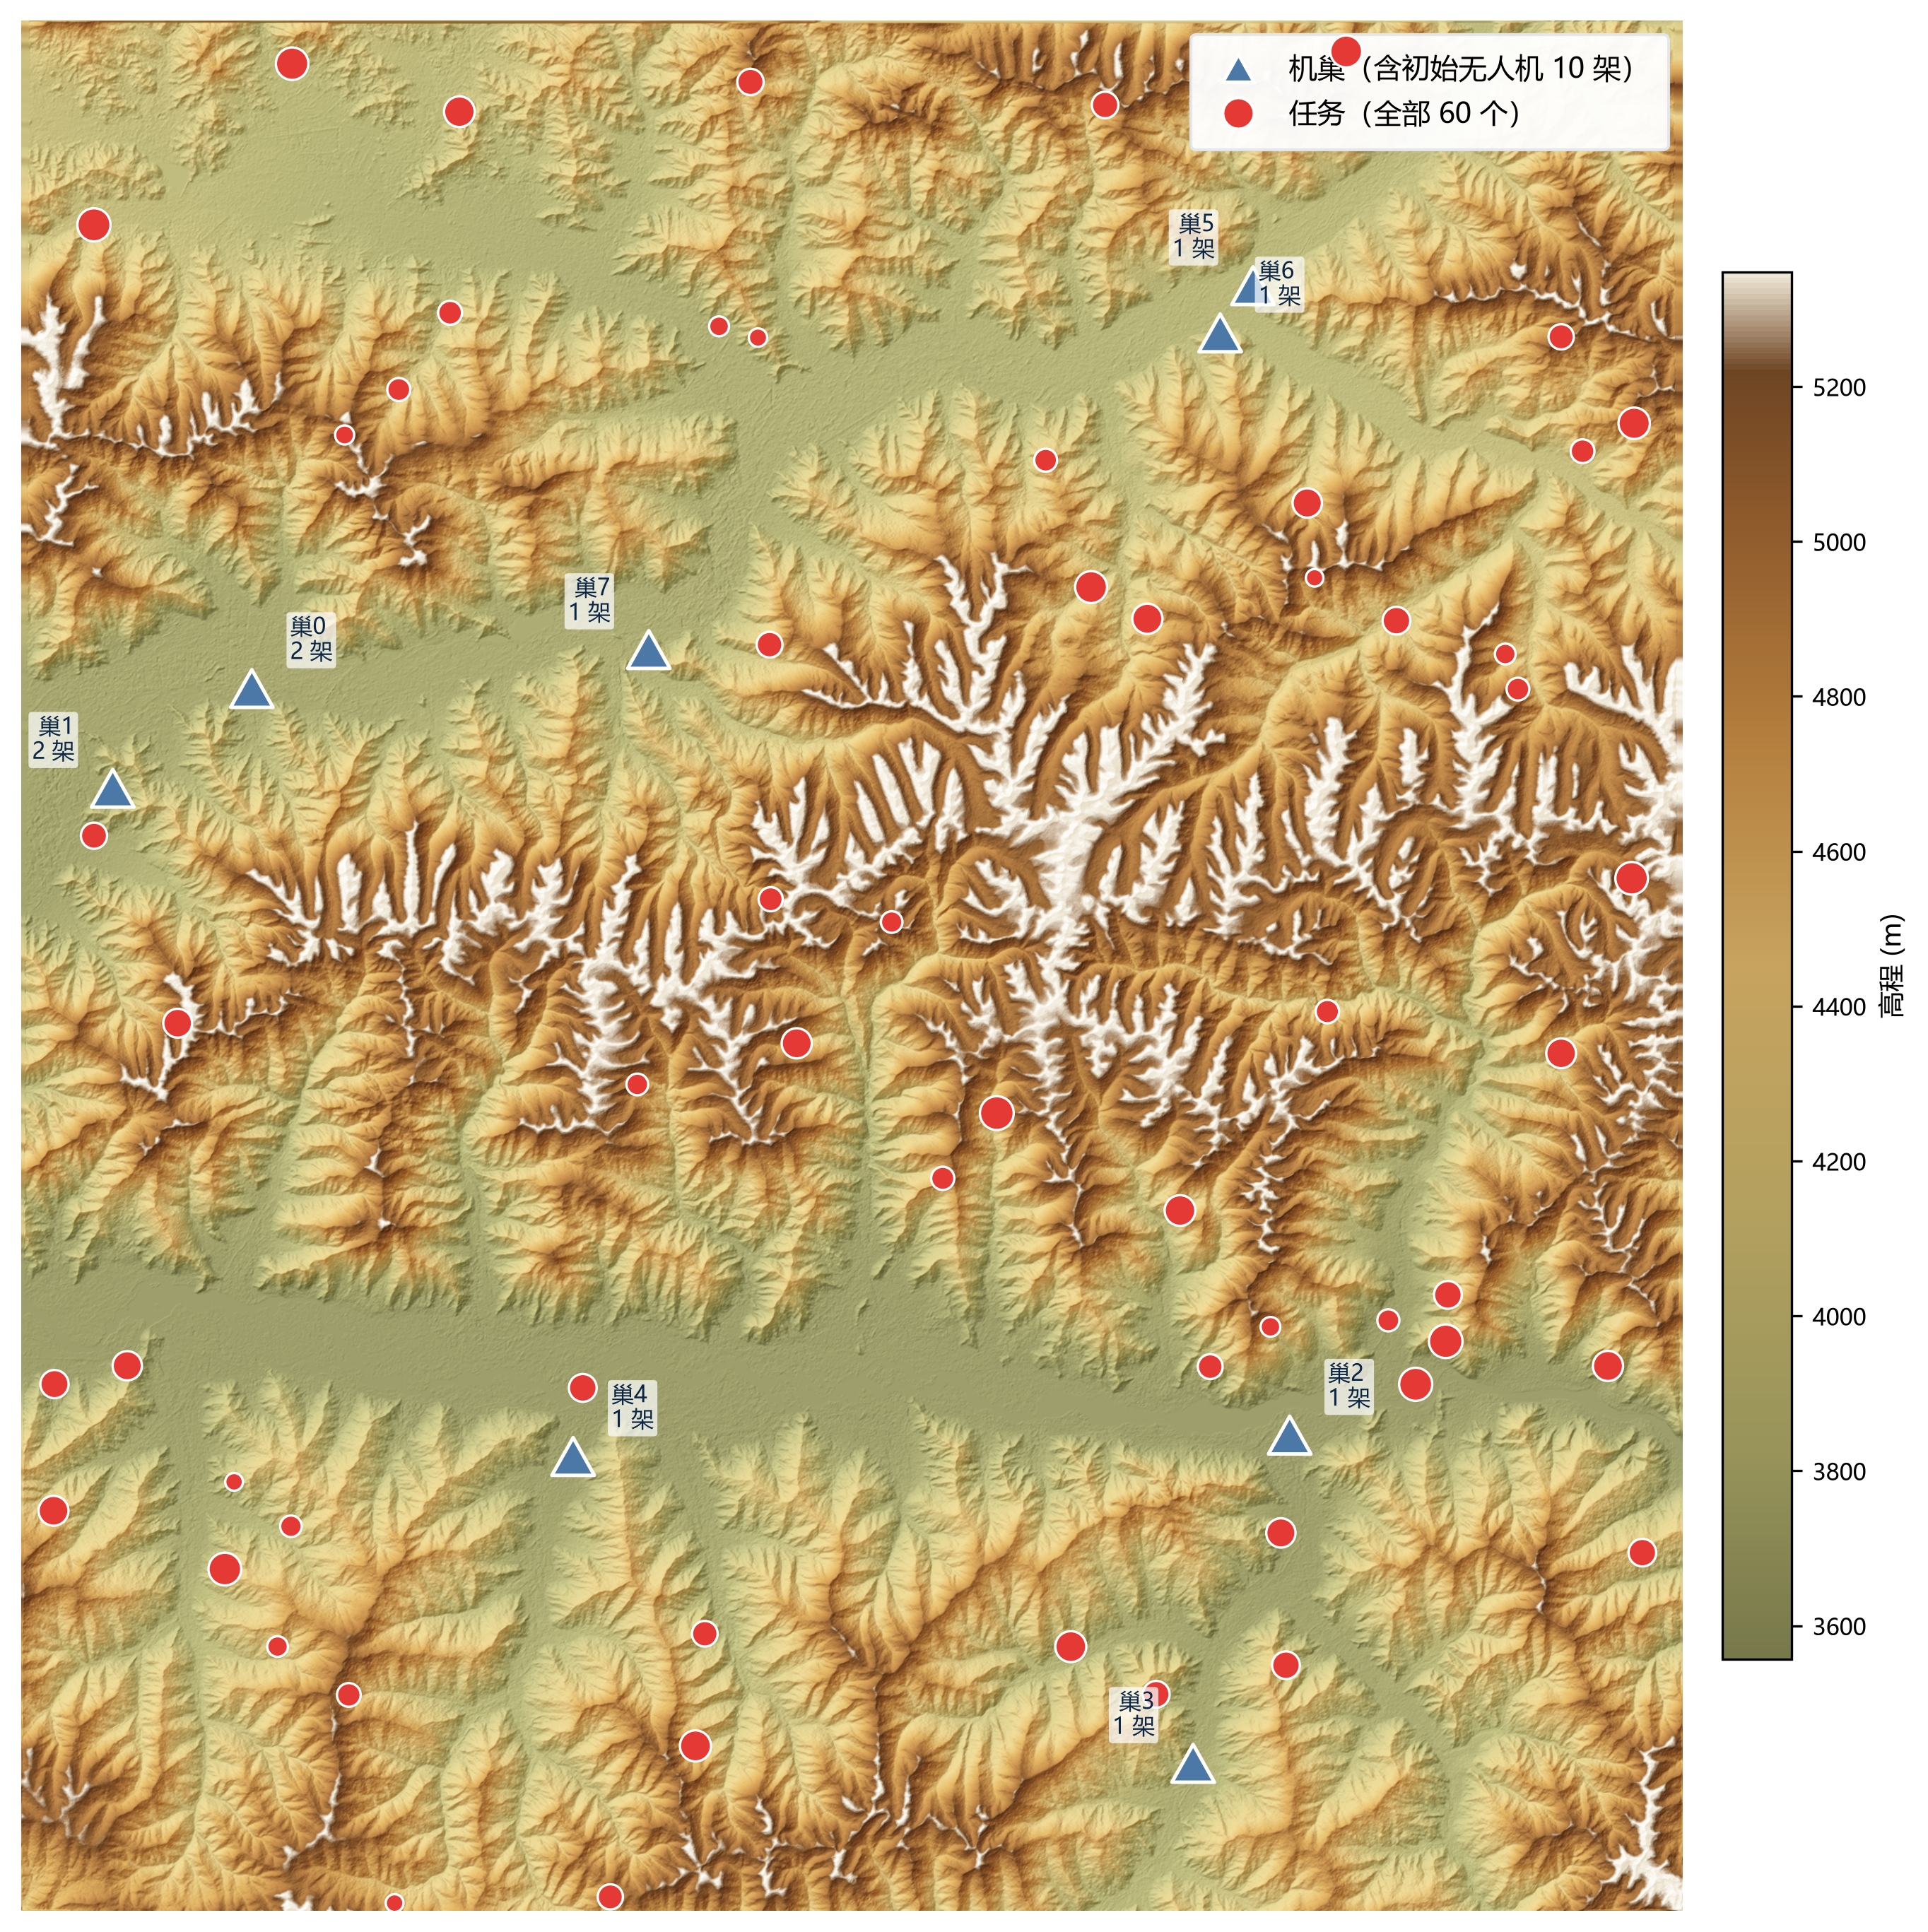
\includegraphics[width=0.92\textwidth]{I01_geo_overview.png}
\caption{场景总览：DEM 地形、8 个机巢位置与 60 个任务的空间分布。
区域跨约 $101.6\times115.0$\,km，机巢跨度约 90\,km。}
\label{fig:geo}
\end{figure}

\begin{figure}[H]
\centering
\begin{minipage}{0.48\textwidth}
  \centering
  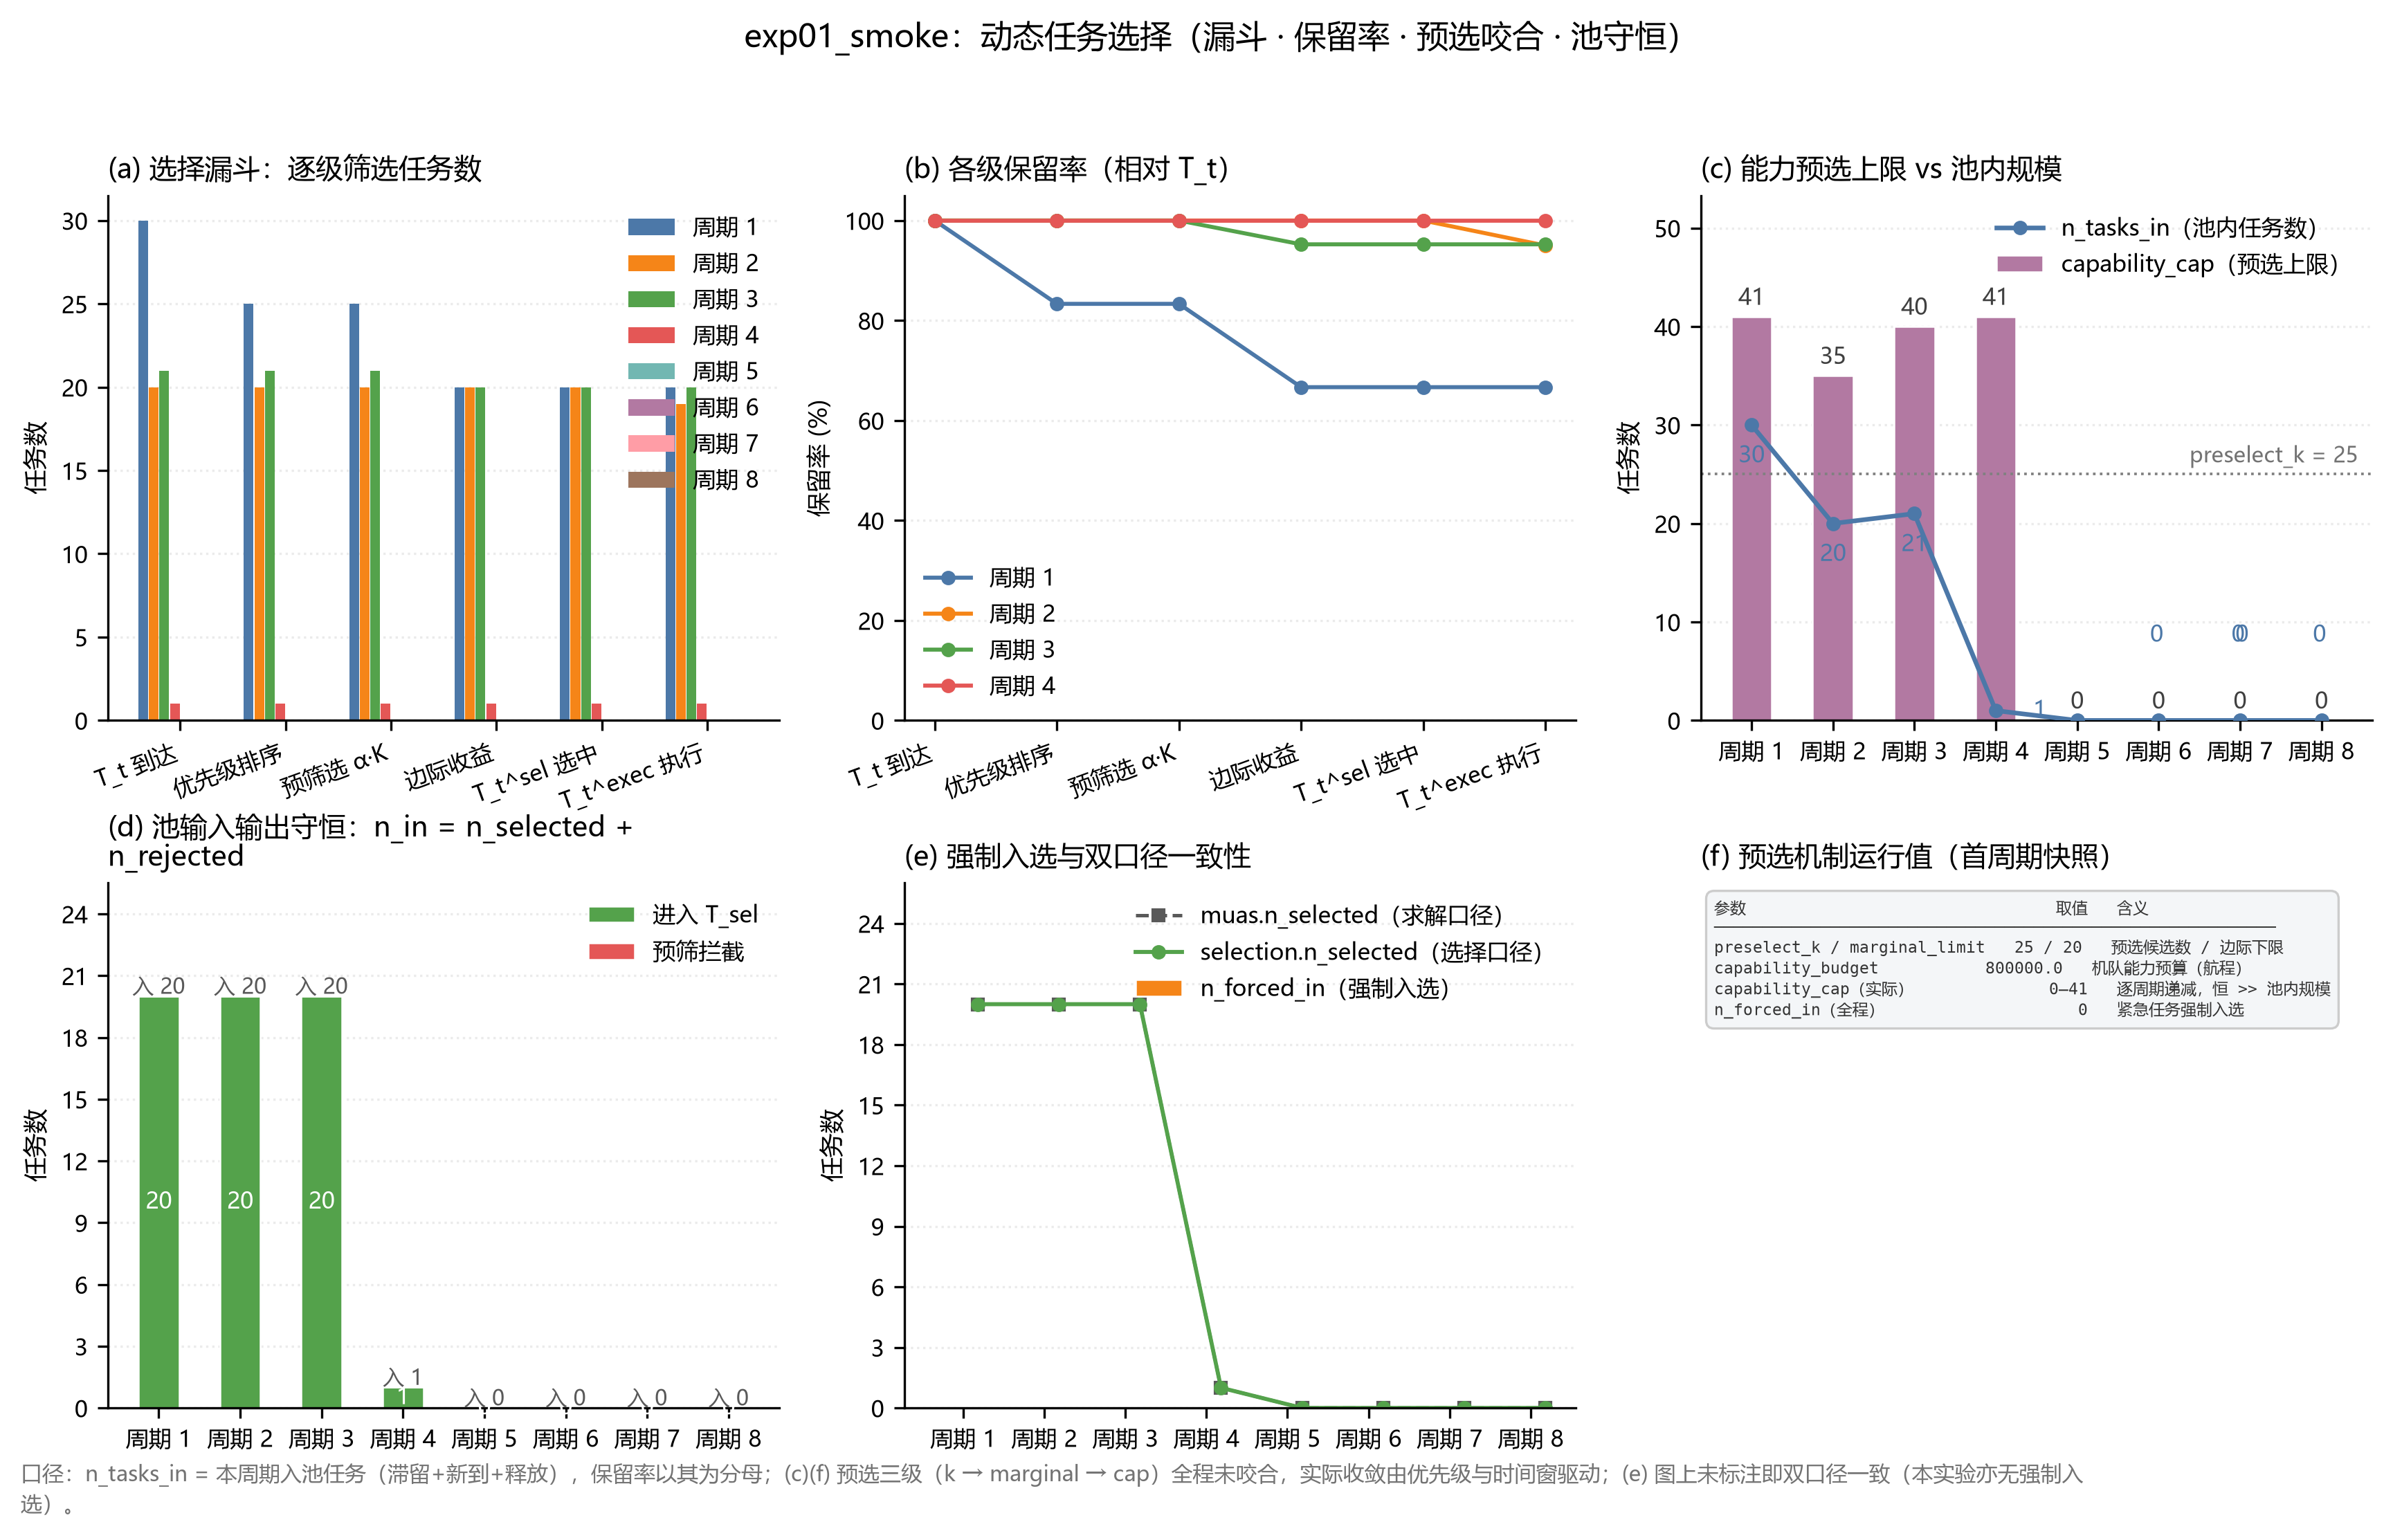
\includegraphics[width=\textwidth]{P01_task_selection.png}
  \caption{任务选择：各周期选中任务数、参与无人机数与顺延情况。}
  \label{fig:sel}
\end{minipage}\hfill
\begin{minipage}{0.48\textwidth}
  \centering
  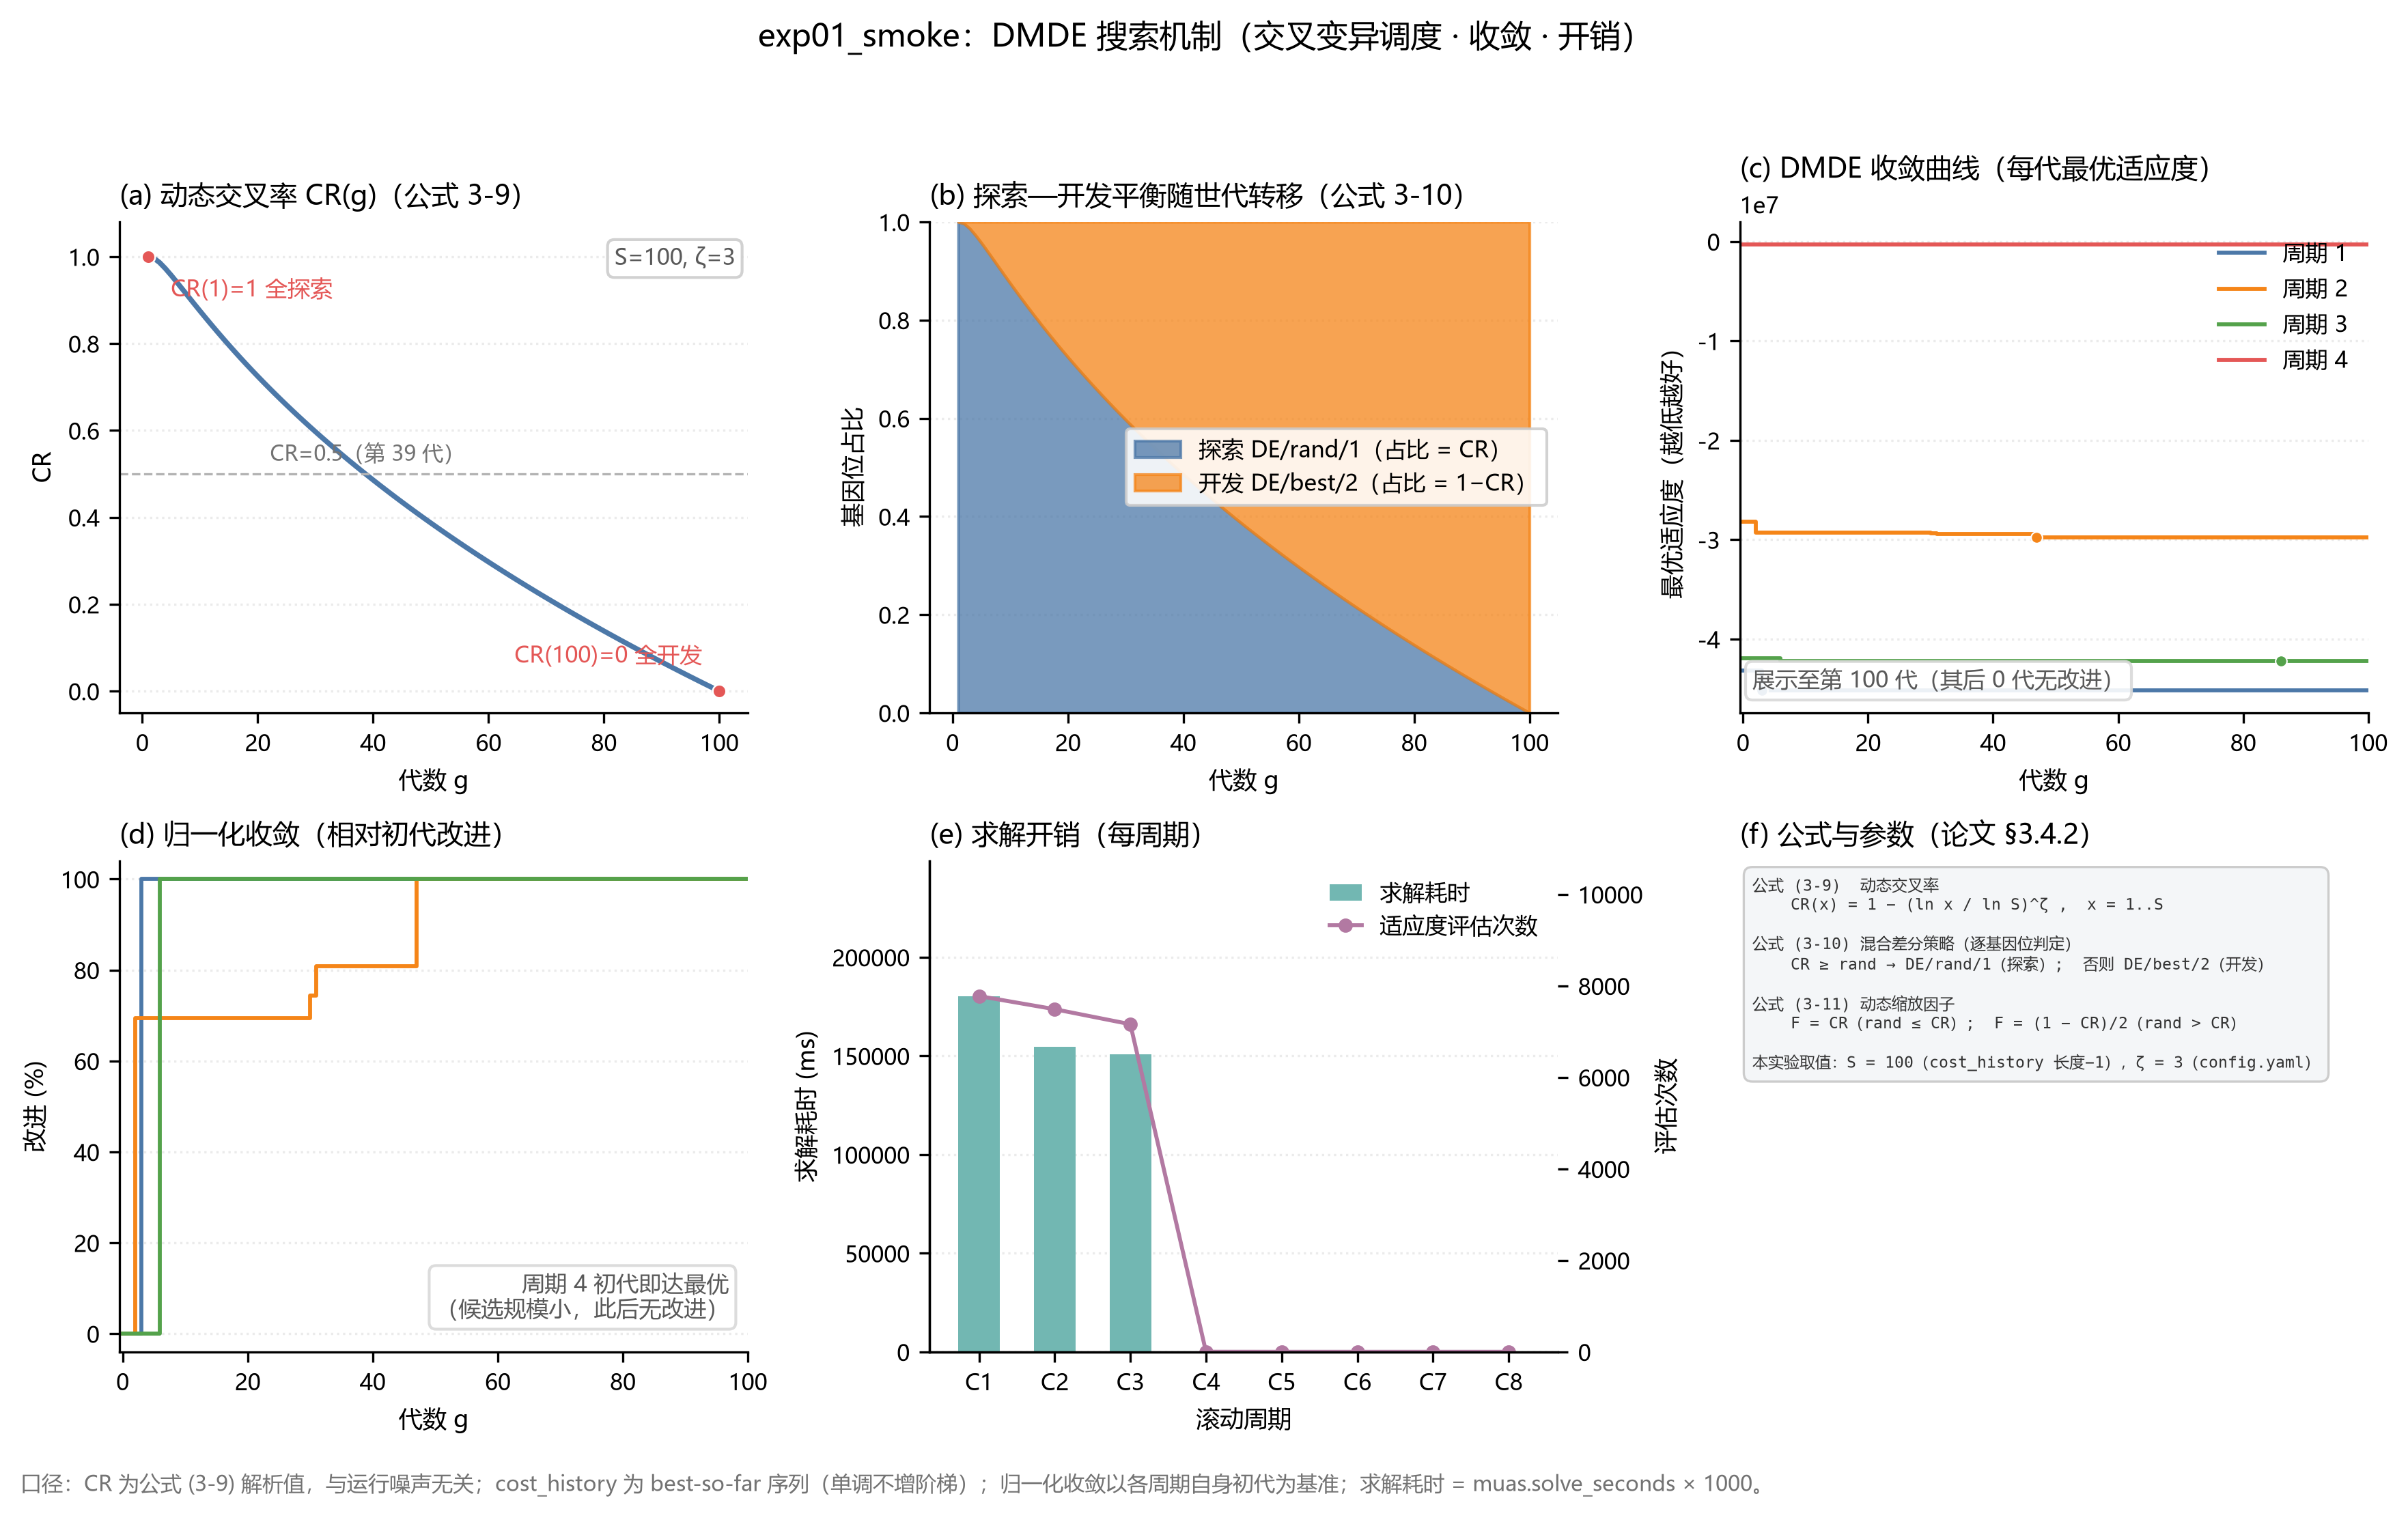
\includegraphics[width=\textwidth]{P02_dmde_search.png}
  \caption{DMDE 搜索过程：适应度收敛曲线与目标分量的演化。}
  \label{fig:dmde}
\end{minipage}
\end{figure}

\subsection{分配结果}

\begin{figure}[H]
\centering
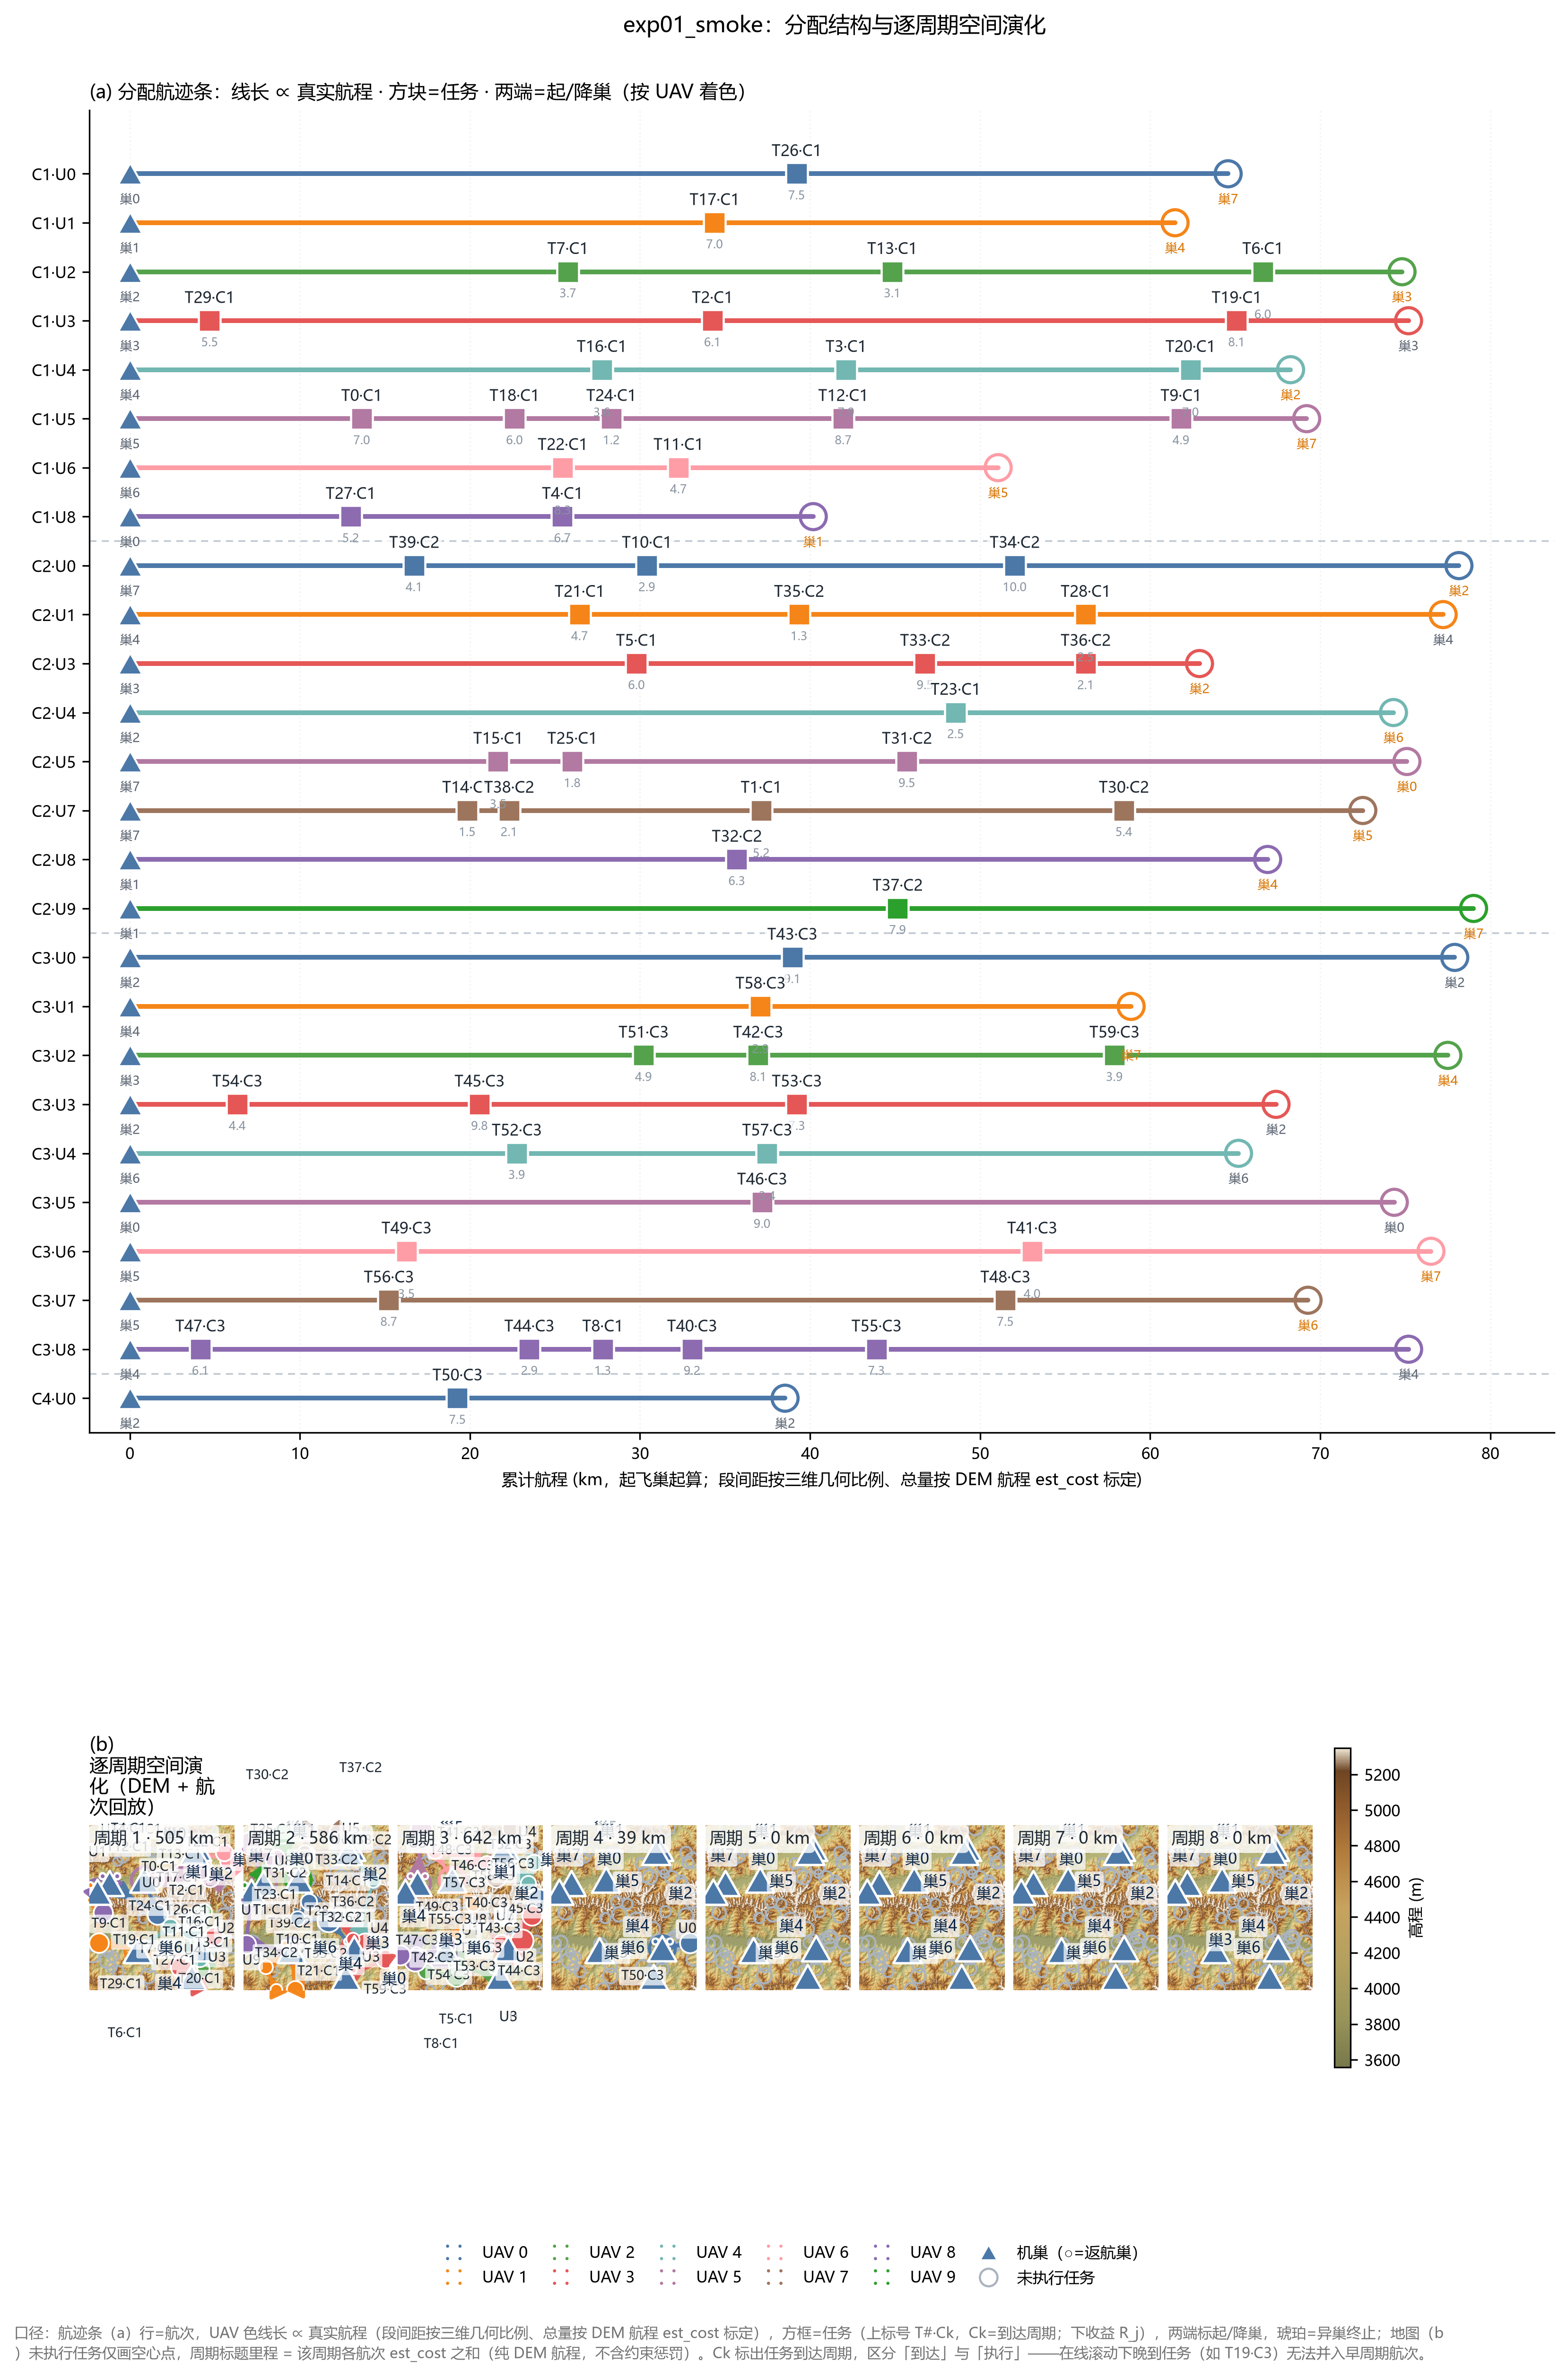
\includegraphics[width=0.92\textwidth]{P03_allocation.png}
\caption{分配结果总览：各无人机的任务归属与访问顺序。}
\label{fig:alloc}
\end{figure}

\begin{figure}[H]
\centering
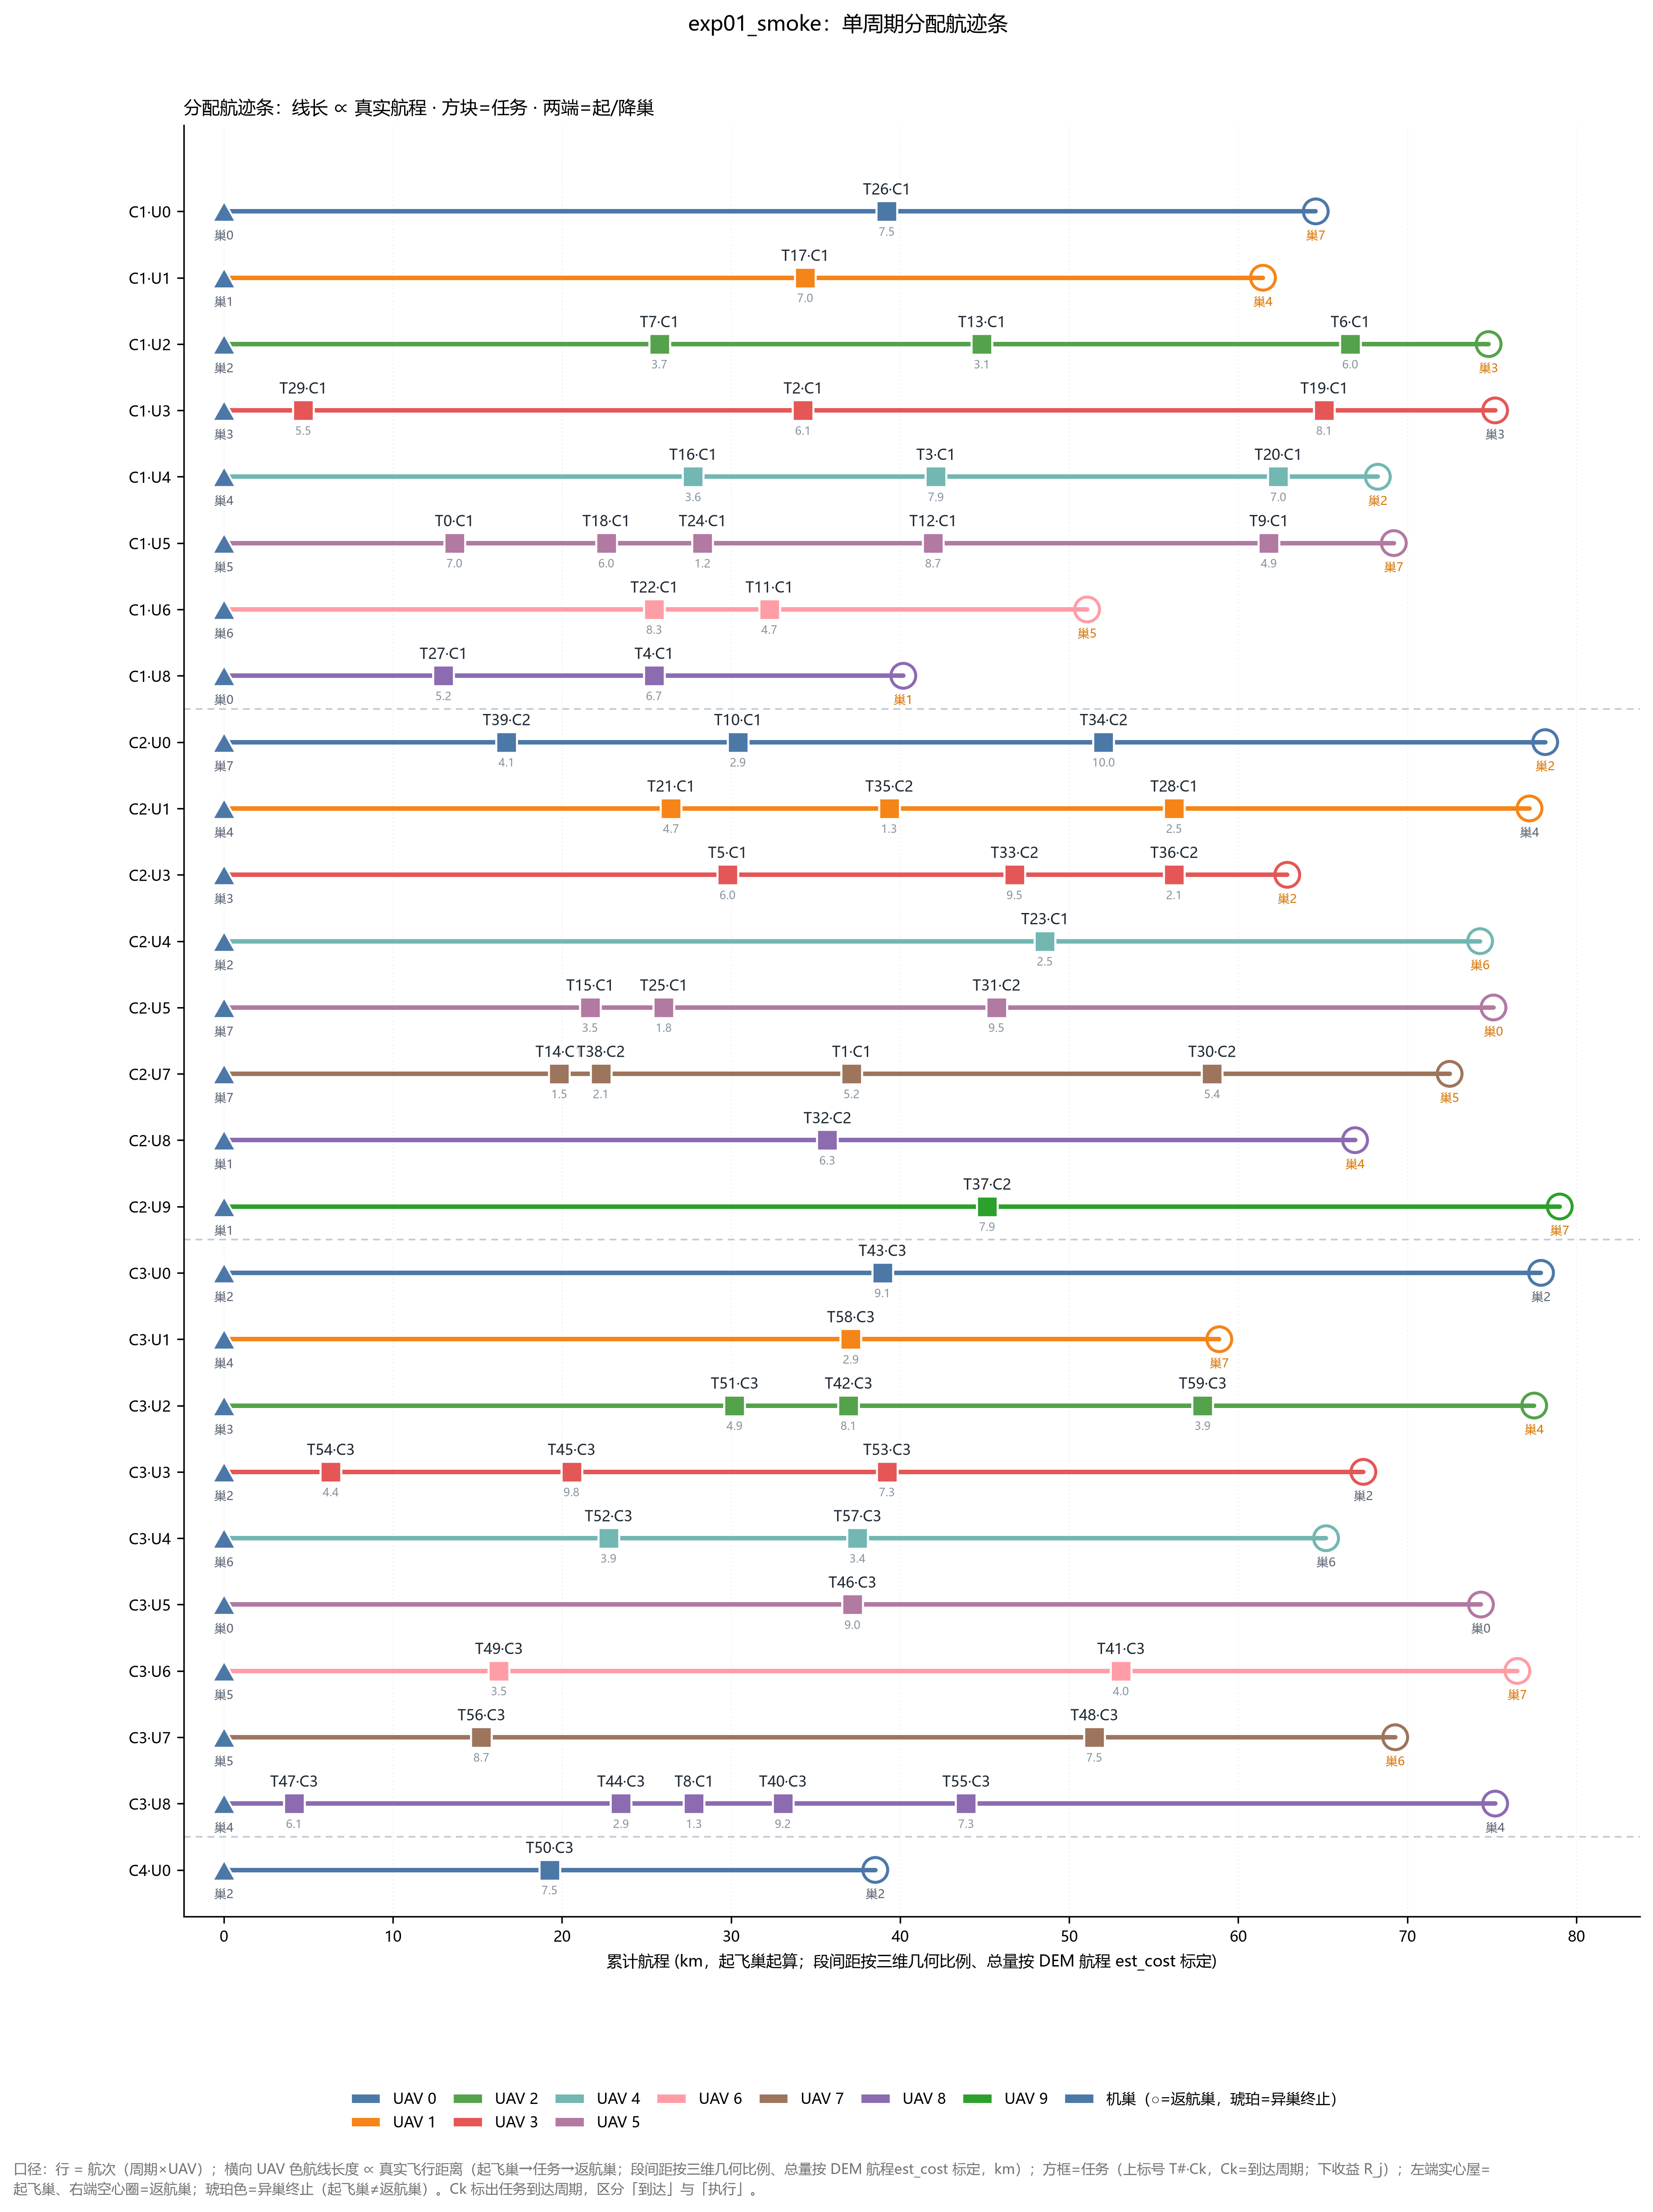
\includegraphics[width=0.92\textwidth]{P04_allocation_gantt.png}
\caption{分配甘特图：各无人机航次的时间占用与任务执行时序，
可看出任务在第 1--3 周期集中执行、第 4 周期收尾。}
\label{fig:gantt}
\end{figure}

\begin{figure}[H]
\centering
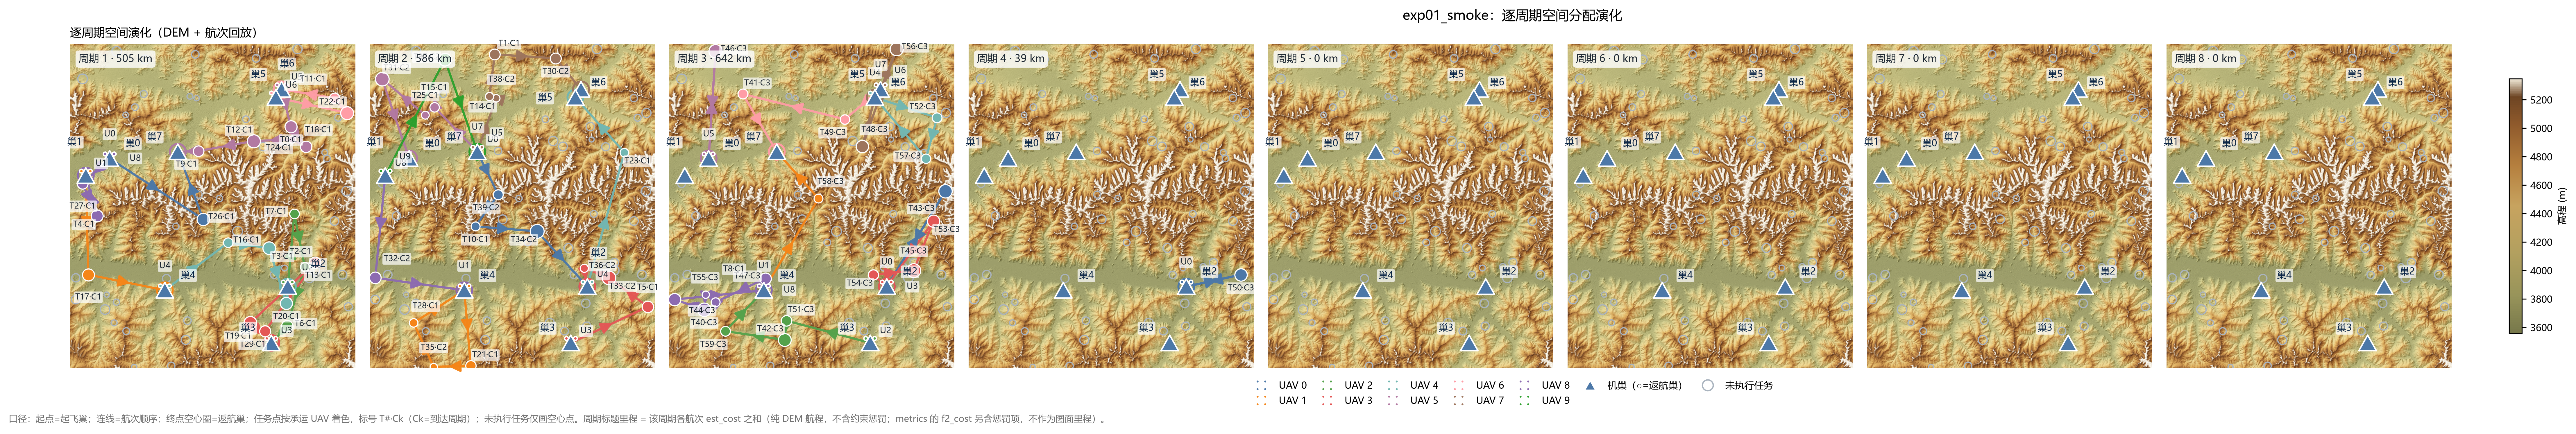
\includegraphics[width=0.92\textwidth]{P05_allocation_map.png}
\caption{分配地图：航次在真实地形上的空间轨迹（含返航腿）。
本图为论文推荐使用的静态分配图。}
\label{fig:map}
\end{figure}

\subsection{状态演化与结果汇总}

\begin{figure}[H]
\centering
\begin{minipage}{0.48\textwidth}
  \centering
  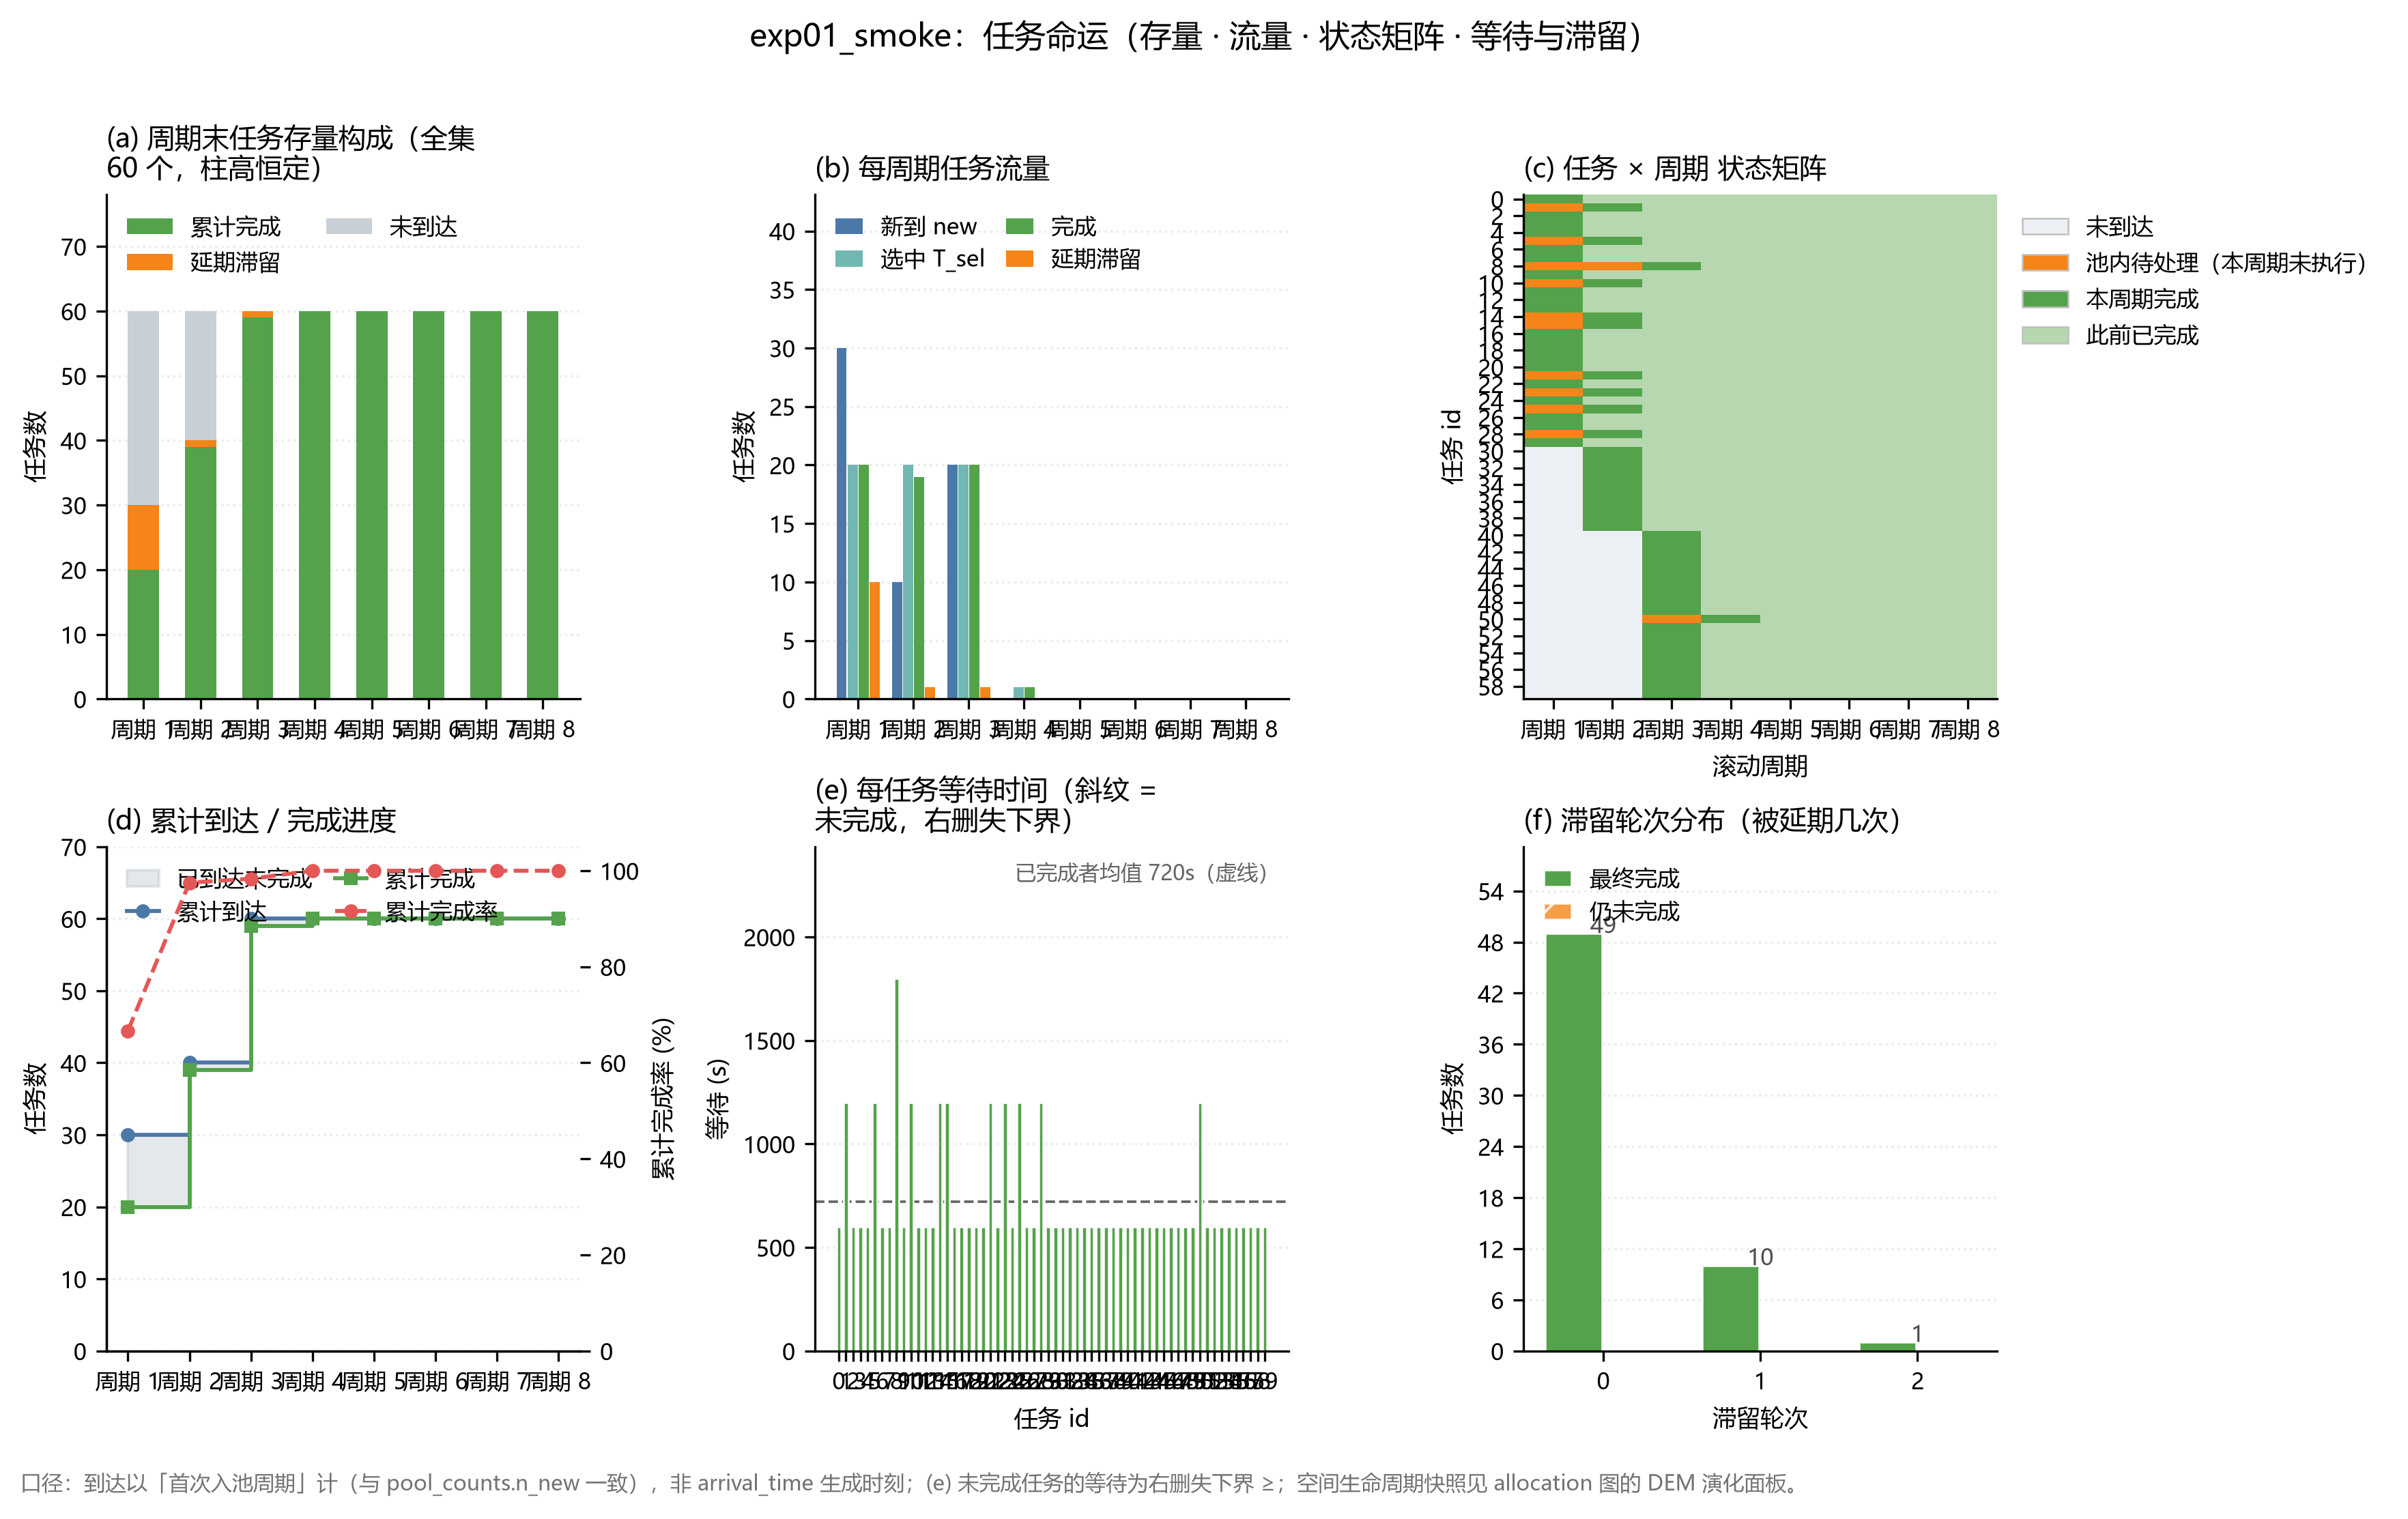
\includegraphics[width=\textwidth]{P09_task_dynamics.png}
  \caption{任务动力学：池内任务数、到达、完成与顺延的逐周期演化。}
  \label{fig:dyn}
\end{minipage}\hfill
\begin{minipage}{0.48\textwidth}
  \centering
  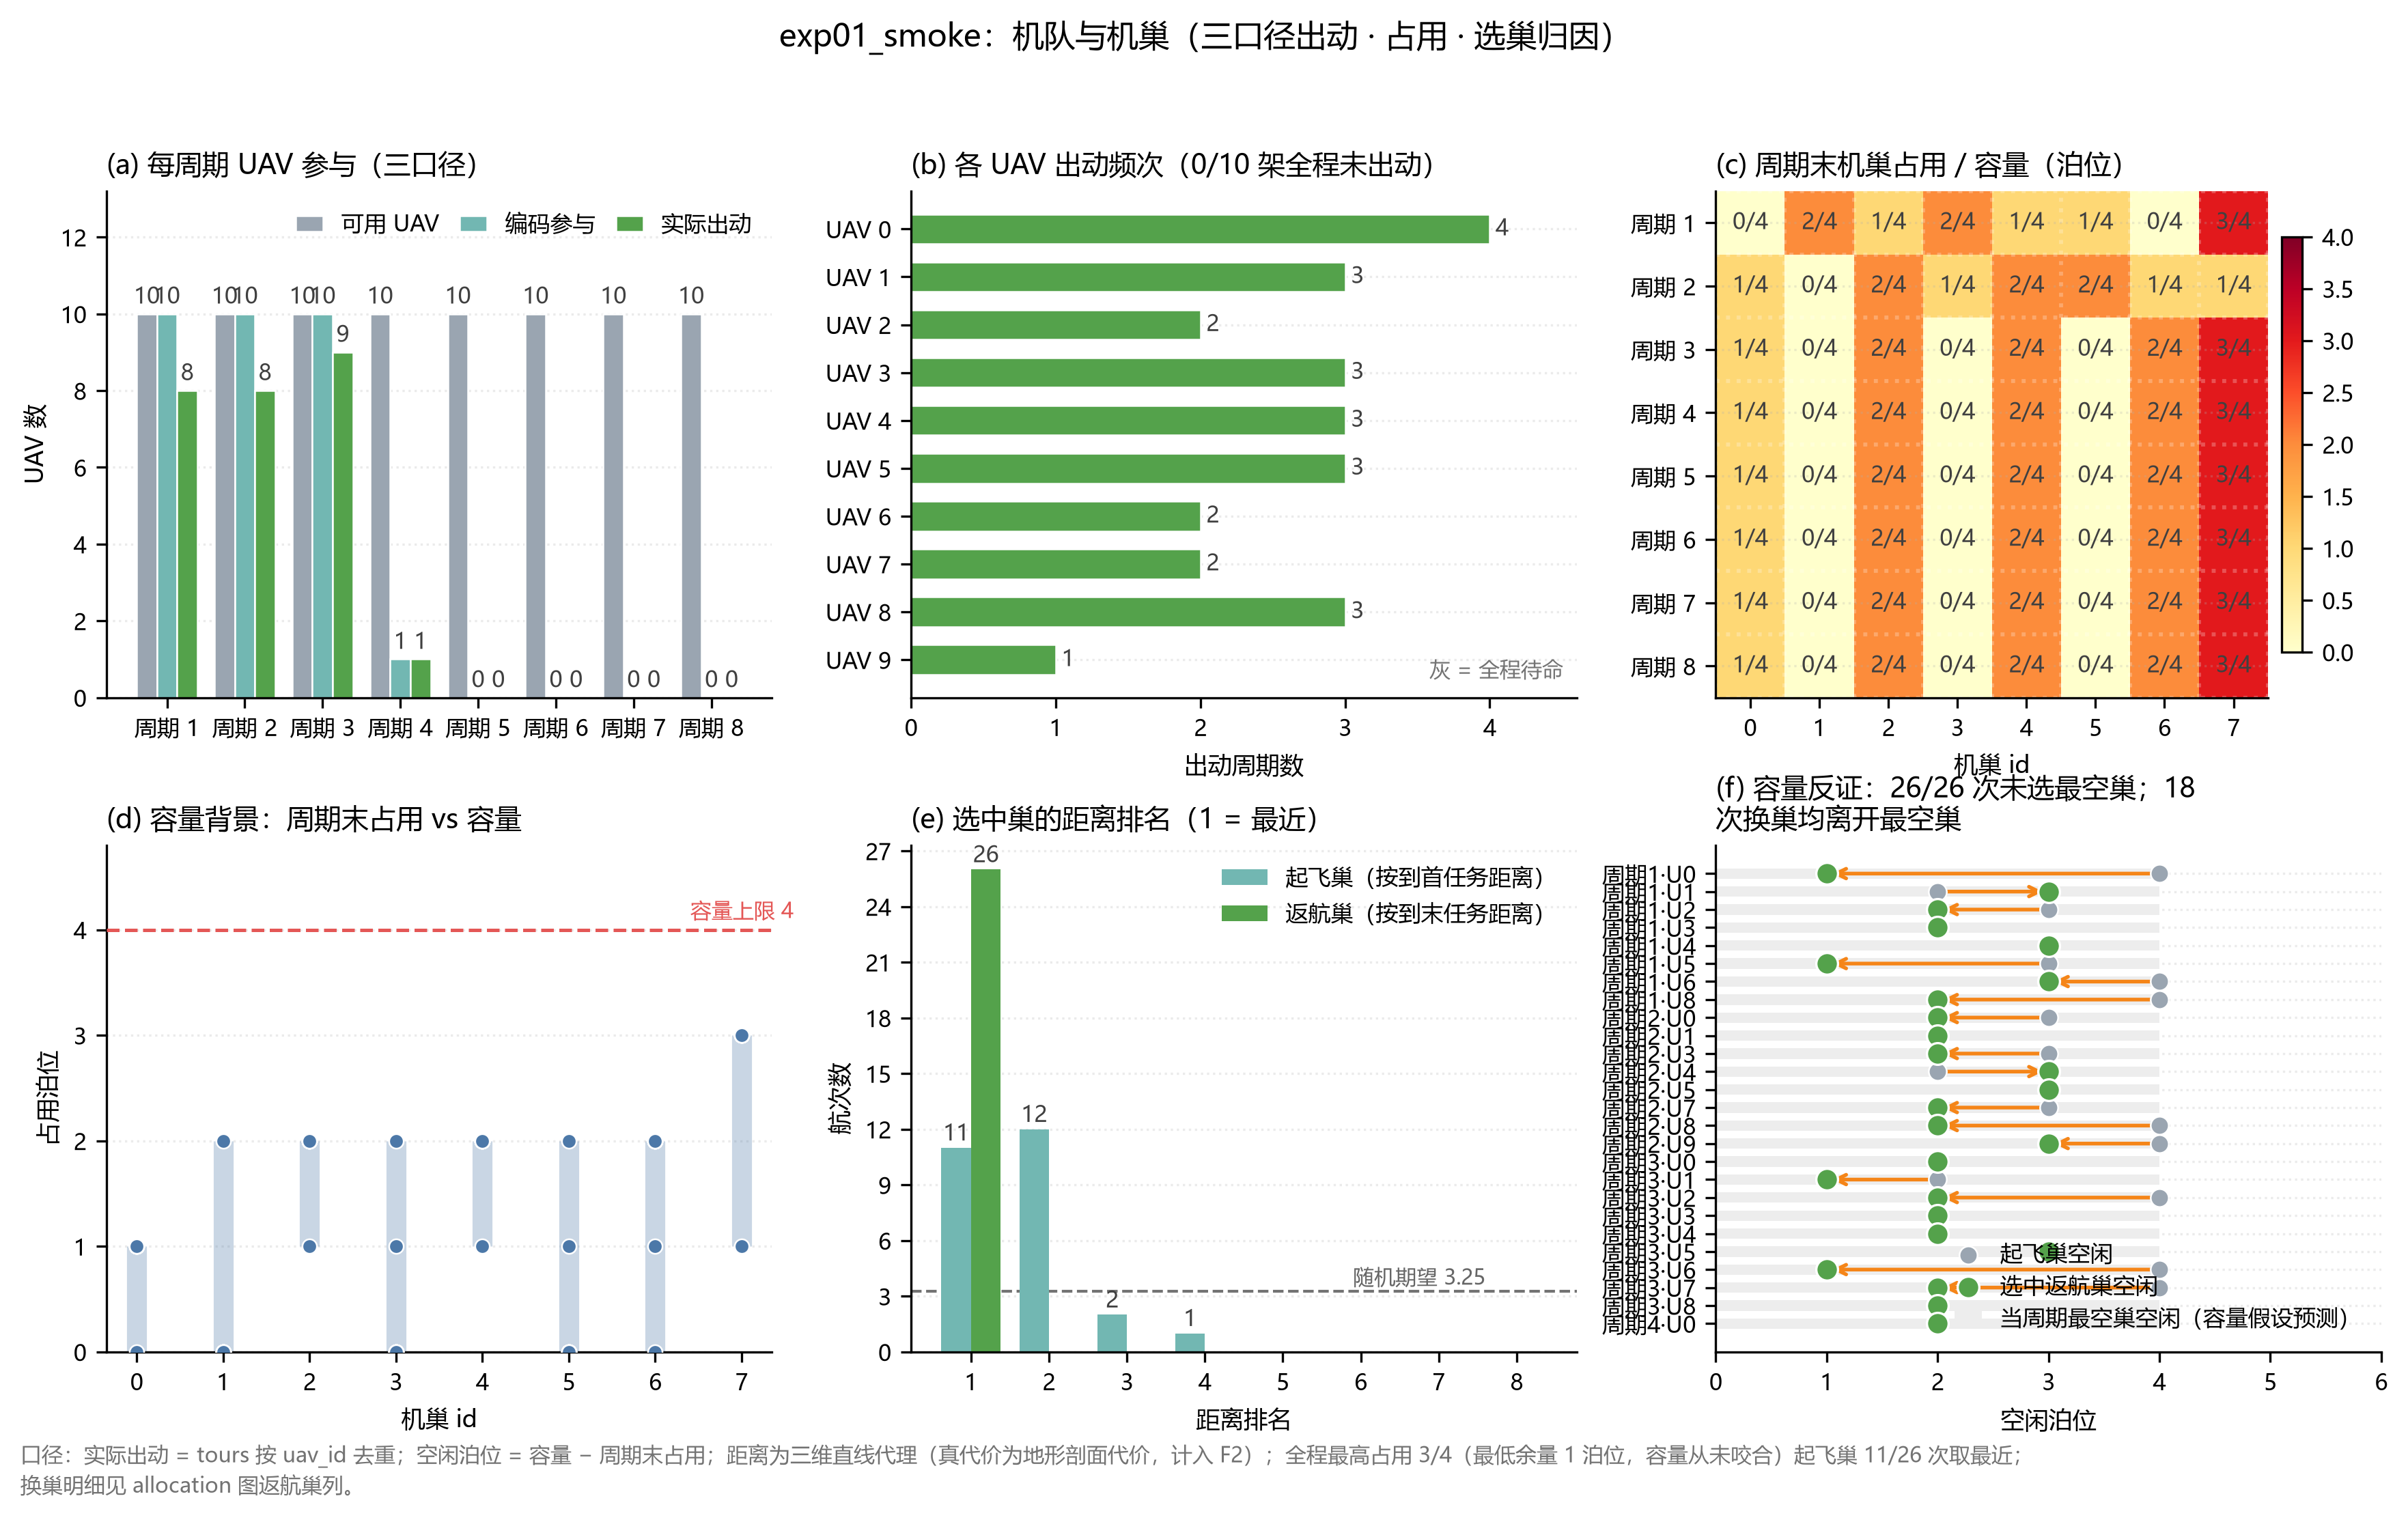
\includegraphics[width=\textwidth]{P10_fleet_state.png}
  \caption{机群状态：可用/忙碌/充电无人机数量与机巢占用的变化。}
  \label{fig:fleet}
\end{minipage}
\end{figure}

\begin{figure}[H]
\centering
\begin{minipage}{0.48\textwidth}
  \centering
  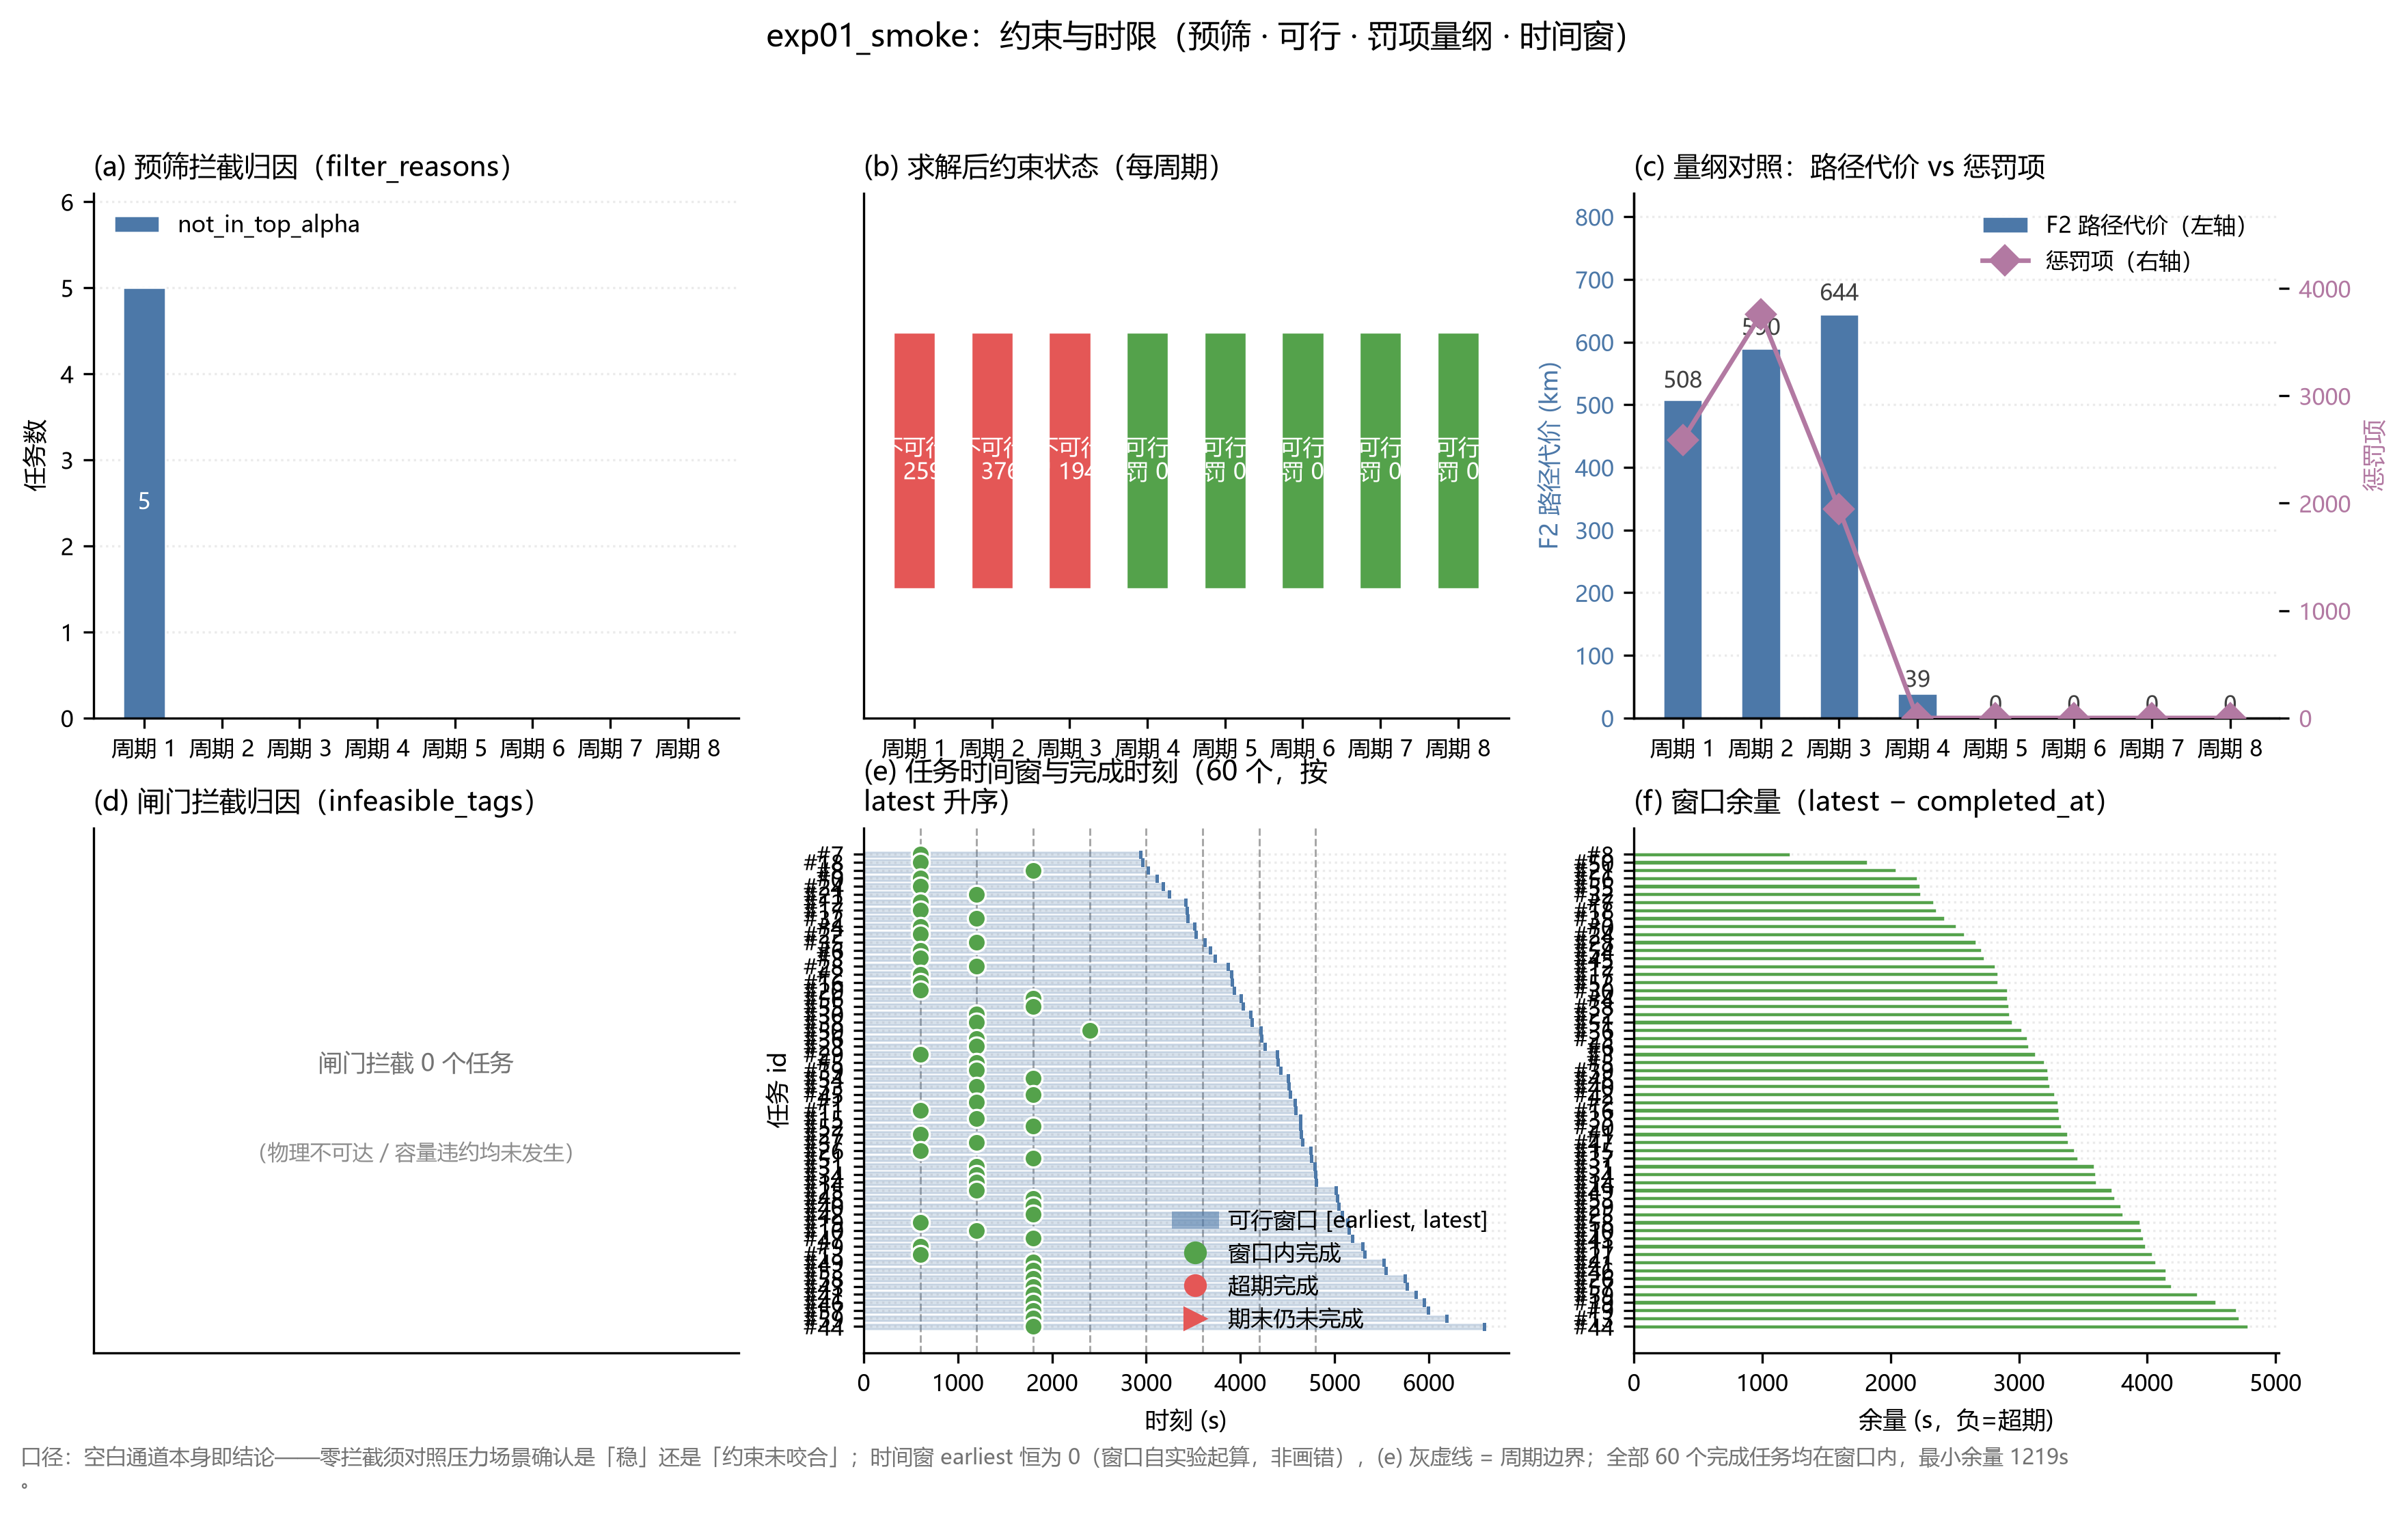
\includegraphics[width=\textwidth]{P11_constraint_state.png}
  \caption{约束状态：航程、时间窗与机巢容量的满足情况。}
  \label{fig:constraint}
\end{minipage}\hfill
\begin{minipage}{0.48\textwidth}
  \centering
  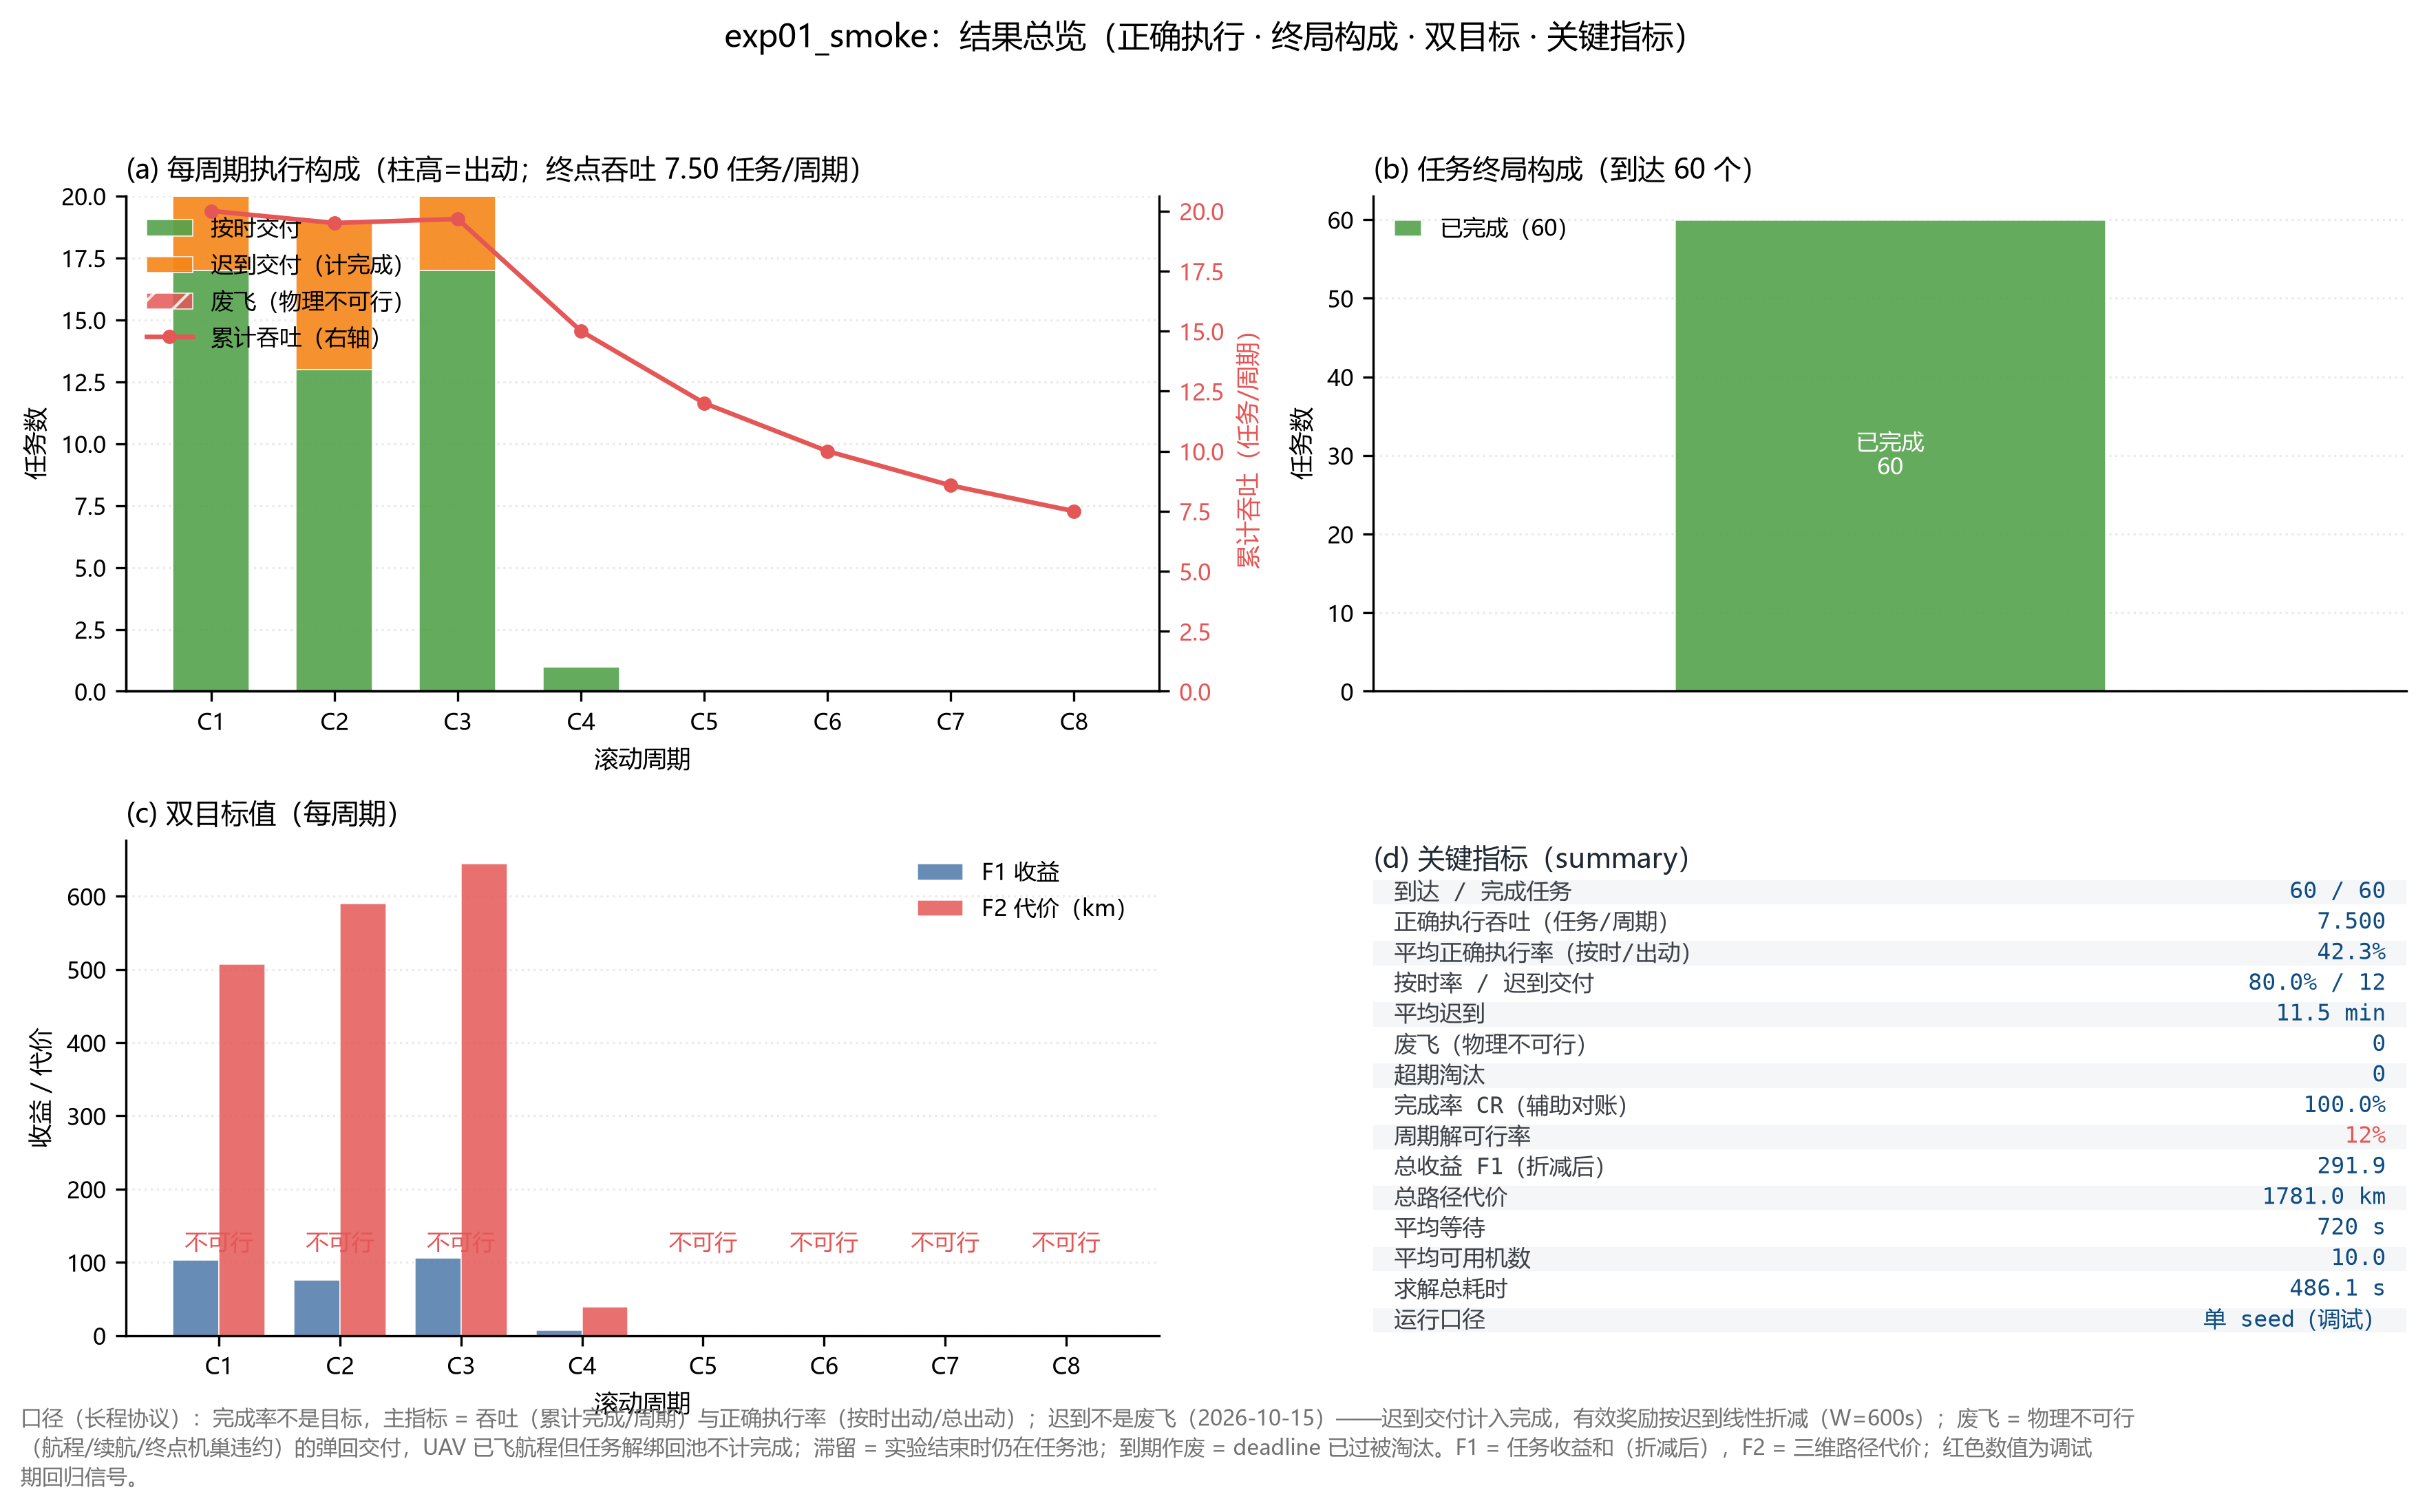
\includegraphics[width=\textwidth]{R01_outcome_summary.png}
  \caption{结果汇总：完成、迟到、废飞、淘汰等核心指标的总体呈现。}
  \label{fig:outcome}
\end{minipage}
\end{figure}

\subsection{动画图件}

以下 3 个动画 GIF 及其末帧海报同样位于 \texttt{results/figures/}，
动态展示分配与执行过程，建议在论文中以其\textbf{末帧海报}作为静态插图：

\begin{table}[H]
\centering
\caption{动画图件清单}
\label{tab:anim}
\footnotesize
\begin{tabular}{@{}ll>{\raggedright\arraybackslash}p{7.2cm}@{}}
\toprule
文件 & 类型 & 内容 \\
\midrule
\texttt{P06\_allocation\_anim.gif} & 动画 & 分配过程逐周期演化 \\
\texttt{P07\_allocation\_status.gif} & 动画 & 机群/任务状态逐周期演化 \\
\texttt{P08\_allocation\_anim\_map.gif} & 动画 & 全周期地图分配动画（约 373\,MB，体积较大） \\
\texttt{P06/P07/P08\_*\_poster.png} & 静态 & 上述动画的末帧海报，可直接用于论文 \\
\bottomrule
\end{tabular}
\end{table}

% ============================================================
\section{附：数据与复现}
% ============================================================

\begin{table}[H]
\centering
\caption{数据文件清单（均位于 \texttt{results/}）}
\label{tab:files}
\small
\begin{tabular}{ll}
\toprule
文件 & 内容 \\
\midrule
\texttt{metrics.json} & 逐周期与汇总指标（本报告全部数值来源） \\
\texttt{solution.json} & 场景、机群、任务、逐周期交付航次 \\
\texttt{run\_meta.json} & 运行元数据（种子、DEM 参数、时间戳） \\
\texttt{figures/} & 17 个图产物 \\
\texttt{tables/exp01\_tables.tex / .pdf} & 结果表（由 \texttt{render\_from\_json.py tables} 生成） \\
\bottomrule
\end{tabular}
\end{table}

复现方式：在本实验目录执行
\fname{python run.py -{}-seeds 42}（默认配置即本报告口径，
\fname{output\_dir: results}）；绘图与表格可在不重跑求解的情况下由
\fname{python render\_from\_json.py png,gif -{}-results results} 与
\fname{python render\_from\_json.py tables -{}-results results} 补出。

\end{document}
